% Options for packages loaded elsewhere
\PassOptionsToPackage{unicode}{hyperref}
\PassOptionsToPackage{hyphens}{url}
%
\documentclass[
  11pt,
]{book}
\title{The Open Science Manual}
\usepackage{etoolbox}
\makeatletter
\providecommand{\subtitle}[1]{% add subtitle to \maketitle
  \apptocmd{\@title}{\par {\large #1 \par}}{}{}
}
\makeatother
\subtitle{Make Your Scientific Research Accessible and Reproducible}
\author{\href{https://claudiozandonella.netlify.app/}{Claudio Zandonella Callegher} and
\href{https://www.linkedin.com/in/davidemassidda/}{Davide Massidda}}
\date{21 April, 2022 {[}last-updated{]}}

\usepackage{amsmath,amssymb}
\usepackage{lmodern}
\usepackage{iftex}
\ifPDFTeX
  \usepackage[T1]{fontenc}
  \usepackage[utf8]{inputenc}
  \usepackage{textcomp} % provide euro and other symbols
\else % if luatex or xetex
  \usepackage{unicode-math}
  \defaultfontfeatures{Scale=MatchLowercase}
  \defaultfontfeatures[\rmfamily]{Ligatures=TeX,Scale=1}
\fi
% Use upquote if available, for straight quotes in verbatim environments
\IfFileExists{upquote.sty}{\usepackage{upquote}}{}
\IfFileExists{microtype.sty}{% use microtype if available
  \usepackage[]{microtype}
  \UseMicrotypeSet[protrusion]{basicmath} % disable protrusion for tt fonts
}{}
\makeatletter
\@ifundefined{KOMAClassName}{% if non-KOMA class
  \IfFileExists{parskip.sty}{%
    \usepackage{parskip}
  }{% else
    \setlength{\parindent}{0pt}
    \setlength{\parskip}{6pt plus 2pt minus 1pt}}
}{% if KOMA class
  \KOMAoptions{parskip=half}}
\makeatother
\usepackage{xcolor}
\IfFileExists{xurl.sty}{\usepackage{xurl}}{} % add URL line breaks if available
\IfFileExists{bookmark.sty}{\usepackage{bookmark}}{\usepackage{hyperref}}
\hypersetup{
  pdftitle={The Open Science Manual},
  hidelinks,
  pdfcreator={LaTeX via pandoc}}
\urlstyle{same} % disable monospaced font for URLs
\usepackage{color}
\usepackage{fancyvrb}
\newcommand{\VerbBar}{|}
\newcommand{\VERB}{\Verb[commandchars=\\\{\}]}
\DefineVerbatimEnvironment{Highlighting}{Verbatim}{commandchars=\\\{\}}
% Add ',fontsize=\small' for more characters per line
\usepackage{framed}
\definecolor{shadecolor}{RGB}{248,248,248}
\newenvironment{Shaded}{\begin{snugshade}}{\end{snugshade}}
\newcommand{\AlertTok}[1]{\textcolor[rgb]{0.94,0.16,0.16}{#1}}
\newcommand{\AnnotationTok}[1]{\textcolor[rgb]{0.56,0.35,0.01}{\textbf{\textit{#1}}}}
\newcommand{\AttributeTok}[1]{\textcolor[rgb]{0.77,0.63,0.00}{#1}}
\newcommand{\BaseNTok}[1]{\textcolor[rgb]{0.00,0.00,0.81}{#1}}
\newcommand{\BuiltInTok}[1]{#1}
\newcommand{\CharTok}[1]{\textcolor[rgb]{0.31,0.60,0.02}{#1}}
\newcommand{\CommentTok}[1]{\textcolor[rgb]{0.56,0.35,0.01}{\textit{#1}}}
\newcommand{\CommentVarTok}[1]{\textcolor[rgb]{0.56,0.35,0.01}{\textbf{\textit{#1}}}}
\newcommand{\ConstantTok}[1]{\textcolor[rgb]{0.00,0.00,0.00}{#1}}
\newcommand{\ControlFlowTok}[1]{\textcolor[rgb]{0.13,0.29,0.53}{\textbf{#1}}}
\newcommand{\DataTypeTok}[1]{\textcolor[rgb]{0.13,0.29,0.53}{#1}}
\newcommand{\DecValTok}[1]{\textcolor[rgb]{0.00,0.00,0.81}{#1}}
\newcommand{\DocumentationTok}[1]{\textcolor[rgb]{0.56,0.35,0.01}{\textbf{\textit{#1}}}}
\newcommand{\ErrorTok}[1]{\textcolor[rgb]{0.64,0.00,0.00}{\textbf{#1}}}
\newcommand{\ExtensionTok}[1]{#1}
\newcommand{\FloatTok}[1]{\textcolor[rgb]{0.00,0.00,0.81}{#1}}
\newcommand{\FunctionTok}[1]{\textcolor[rgb]{0.00,0.00,0.00}{#1}}
\newcommand{\ImportTok}[1]{#1}
\newcommand{\InformationTok}[1]{\textcolor[rgb]{0.56,0.35,0.01}{\textbf{\textit{#1}}}}
\newcommand{\KeywordTok}[1]{\textcolor[rgb]{0.13,0.29,0.53}{\textbf{#1}}}
\newcommand{\NormalTok}[1]{#1}
\newcommand{\OperatorTok}[1]{\textcolor[rgb]{0.81,0.36,0.00}{\textbf{#1}}}
\newcommand{\OtherTok}[1]{\textcolor[rgb]{0.56,0.35,0.01}{#1}}
\newcommand{\PreprocessorTok}[1]{\textcolor[rgb]{0.56,0.35,0.01}{\textit{#1}}}
\newcommand{\RegionMarkerTok}[1]{#1}
\newcommand{\SpecialCharTok}[1]{\textcolor[rgb]{0.00,0.00,0.00}{#1}}
\newcommand{\SpecialStringTok}[1]{\textcolor[rgb]{0.31,0.60,0.02}{#1}}
\newcommand{\StringTok}[1]{\textcolor[rgb]{0.31,0.60,0.02}{#1}}
\newcommand{\VariableTok}[1]{\textcolor[rgb]{0.00,0.00,0.00}{#1}}
\newcommand{\VerbatimStringTok}[1]{\textcolor[rgb]{0.31,0.60,0.02}{#1}}
\newcommand{\WarningTok}[1]{\textcolor[rgb]{0.56,0.35,0.01}{\textbf{\textit{#1}}}}
\usepackage{longtable,booktabs,array}
\usepackage{calc} % for calculating minipage widths
% Correct order of tables after \paragraph or \subparagraph
\usepackage{etoolbox}
\makeatletter
\patchcmd\longtable{\par}{\if@noskipsec\mbox{}\fi\par}{}{}
\makeatother
% Allow footnotes in longtable head/foot
\IfFileExists{footnotehyper.sty}{\usepackage{footnotehyper}}{\usepackage{footnote}}
\makesavenoteenv{longtable}
\usepackage{graphicx}
\makeatletter
\def\maxwidth{\ifdim\Gin@nat@width>\linewidth\linewidth\else\Gin@nat@width\fi}
\def\maxheight{\ifdim\Gin@nat@height>\textheight\textheight\else\Gin@nat@height\fi}
\makeatother
% Scale images if necessary, so that they will not overflow the page
% margins by default, and it is still possible to overwrite the defaults
% using explicit options in \includegraphics[width, height, ...]{}
\setkeys{Gin}{width=\maxwidth,height=\maxheight,keepaspectratio}
% Set default figure placement to htbp
\makeatletter
\def\fps@figure{htbp}
\makeatother
\setlength{\emergencystretch}{3em} % prevent overfull lines
\providecommand{\tightlist}{%
  \setlength{\itemsep}{0pt}\setlength{\parskip}{0pt}}
\setcounter{secnumdepth}{5}
\newlength{\cslhangindent}
\setlength{\cslhangindent}{1.5em}
\newlength{\csllabelwidth}
\setlength{\csllabelwidth}{3em}
\newlength{\cslentryspacingunit} % times entry-spacing
\setlength{\cslentryspacingunit}{\parskip}
\newenvironment{CSLReferences}[2] % #1 hanging-ident, #2 entry spacing
 {% don't indent paragraphs
  \setlength{\parindent}{0pt}
  % turn on hanging indent if param 1 is 1
  \ifodd #1
  \let\oldpar\par
  \def\par{\hangindent=\cslhangindent\oldpar}
  \fi
  % set entry spacing
  \setlength{\parskip}{#2\cslentryspacingunit}
 }%
 {}
\usepackage{calc}
\newcommand{\CSLBlock}[1]{#1\hfill\break}
\newcommand{\CSLLeftMargin}[1]{\parbox[t]{\csllabelwidth}{#1}}
\newcommand{\CSLRightInline}[1]{\parbox[t]{\linewidth - \csllabelwidth}{#1}\break}
\newcommand{\CSLIndent}[1]{\hspace{\cslhangindent}#1}
%----------------------------%
%----    preamble.tex    ----%
%----------------------------%

\usepackage{booktabs}
\usepackage{amsthm}
\makeatletter
\def\thm@space@setup{%
  \thm@preskip=8pt plus 2pt minus 4pt
  \thm@postskip=\thm@preskip
}
\makeatother

%----    layout    ----%

% change margins
\usepackage[outer = 105pt, inner = 85pt]{geometry}
\usepackage{afterpage}
\voffset 5pt
\headsep 29pt
\footskip 35pt
\textheight 590pt
\usepackage{layout}% http://ctan.org/pkg/layouts

% caption
\usepackage[labelfont=bf]{caption}


%---- page numbers header and footer
\usepackage{xcolor}

\definecolor{ctcolorgraylight}{RGB}{153, 153, 153}
\definecolor{ctcolorgray}{RGB}{120, 120, 120}

\usepackage{fancyhdr}
\usepackage[fit]{truncate}

% Redefine the plain page style
\fancypagestyle{plain}{%
  \fancyhf{}%
  \fancyfoot[LE,RO]{\textcolor{ctcolorgray}{\thepage}}
  \renewcommand{\headrulewidth}{0pt}% Line at the header invisible
}

% fancy style
\fancypagestyle{myfancy}{%
  \fancyhf{}
  \fancyhead[LE]{\footnotesize\textit{\nouppercase{\truncate{0.98\headwidth}{\textcolor{ctcolorgray}{\rightmark}}}}}
  \fancyhead[RO]{\footnotesize\textit{\truncate{0.98\headwidth}{\textcolor{ctcolorgray}{\leftmark}}}}
  \fancyfoot[LE,RO]{\textcolor{ctcolorgray}{\thepage}}
  \renewcommand{\headrulewidth}{1.5pt}
  \renewcommand{\headrule}{\hbox to\headwidth{%
      \color{ctcolorgraylight}\leaders\hrule height \headrulewidth\hfill}}
}

% part page style
\newcommand{\cpart}[1]{
\cleardoublepage
\stepcounter{part}
\pagestyle{empty}
\begin{flushright}
  \vspace*{2.5cm}
  {\fontfamily{pnc}\fontsize{75}{80}\selectfont%
   \textcolor{ctcolorgraylight}{\textbf{Part \thepart}}\par}%
  \vspace*{1cm}
  {\Huge\textbf{#1}}%
  \end{flushright}
\addcontentsline{toc}{part}{Part \thepart\hspace{1em}#1}
\cleardoublepage
\pagestyle{plain}
}

\usepackage{titletoc}
\titlecontents{part}[0pt]{\bfseries\protect\addvspace{20pt}\titlerule\addvspace{.7ex}}%
{}{}%% numbered/numberless formatting
{}%% to be replaced with {} if you don't want any page number for parts
[\addvspace{0.7ex}\titlerule\addvspace{1.5ex}]

%---- chapter title
\usepackage[newcentury]{quotchap}

\makeatletter
\renewcommand*{\chapnumfont}{%
  \usefont{T1}{\@defaultcnfont}{b}{n}\fontsize{120}{150}\selectfont% Default: 100/130
  \color{chaptergrey}%
}
\makeatother


%----    define infoboxes    ----%
\usepackage[skins, most]{tcolorbox}

% colors
\definecolor{background}{HTML}{fcfcfc}
\definecolor{tip-text}{HTML}{e7b002}
\definecolor{tip-line}{HTML}{fdce38}
\definecolor{warning-text}{HTML}{b06336}
\definecolor{warning-line}{HTML}{c97d50}
\definecolor{deffun-text}{HTML}{0b797e}
\definecolor{deffun-line}{HTML}{6CC2C9}
\definecolor{design-text}{HTML}{7c972e}
\definecolor{design-line}{HTML}{a7c84a}
\definecolor{trick-text}{HTML}{8c3031}
\definecolor{trick-line}{HTML}{A3595A}

\newtcolorbox{mybox}[1][black]{
  colback=background,
  coltext=black,
  colframe=#1,
  boxsep=5pt,
  arc=4pt,
  breakable}

% tip
\newenvironment{tip}[1][Title]
  {
  \setlength{\fboxsep}{1em}
  \begin{mybox}[tip-line]
    \raisebox{-.2\height}{
\includegraphics[height=.6cm]{assets/images/lightbulb.png}} \large \textcolor{tip-text}{Tip-Box: #1\\\vspace*{.5em}}\normalsize
    }
    {
  \end{mybox}
  }

% warnings
\newenvironment{warning}[1][Title]
  {
  \setlength{\fboxsep}{1em}
  \begin{mybox}[warning-line]
    \raisebox{-.2\height}{
\includegraphics[height=.6cm]{assets/images/gotcha.png}} \large \textcolor{warning-text}{Warning-Box: #1\\\vspace*{.5em}}\normalsize
    }
    {
  \end{mybox}
  }

% deffun
\newenvironment{deffun}[1][Title]
  {
  \setlength{\fboxsep}{1em}
  \begin{mybox}[deffun-line]
    \raisebox{-.2\height}{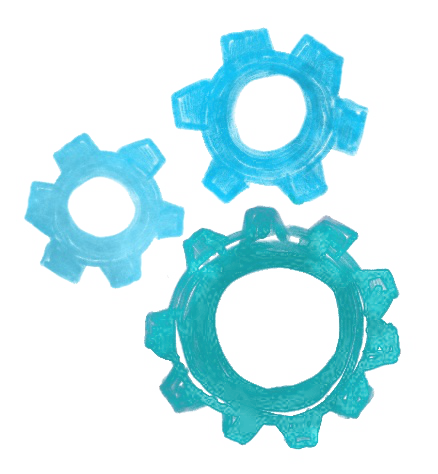
\includegraphics[height=.6cm]{assets/images/gears.png}} \large \textcolor{deffun-text}{Definition-Box: #1\\\vspace*{.5em}}\normalsize
    }
    {
  \end{mybox}
  }

% doclinks
\newenvironment{doclinks}
  {
  \setlength{\fboxsep}{1em}
  \begin{mybox}[deffun-line]
    \raisebox{-.2\height}{
\includegraphics[height=.6cm]{assets/images/doc-links.png}} \large \textcolor{deffun-text}{Documentation-Box}\vspace*{.5em}\normalsize
    }
    {
  \end{mybox}
  }

% design
\newenvironment{design}[1][Title]
  {
  \setlength{\fboxsep}{1em}
  \begin{mybox}[design-line]
    \raisebox{-.2\height}{
\includegraphics[height=.6cm]{assets/images/design.png}} \large \textcolor{design-text}{Details-Box: #1\\\vspace*{.5em}}\normalsize
    }
    {
  \end{mybox}
  }

% trick
\newenvironment{trick}[1][Title]
  {
  \setlength{\fboxsep}{1em}
  \begin{mybox}[trick-line]
    \raisebox{-.2\height}{
\includegraphics[height=.6cm]{assets/images/hat.png}} \large \textcolor{trick-text}{Trick-Box: #1\\\vspace*{.5em}}\normalsize
    }
    {
  \end{mybox}
  }

%----    quote


\definecolor{block-gray}{gray}{0.95}


\newtcolorbox{line-left}{%
    colback=white,
    % grow to right by=-10mm,
    % grow to left by=-10mm,
    boxrule=0pt,
    boxsep=0pt,
    breakable,
    enhanced jigsaw,
    borderline west={2pt}{0pt}{gray},
    borderline north={0pt}{0pt}{white},
    borderline south={0pt}{0pt}{white},
    % title={#2\par},
    % colbacktitle={block-gray},
    % coltitle={black},
    % fonttitle={\large\bfseries},
    % attach title to upper={},
    % #1,
}

% \renewenvironment{quote}
%                {\begin{line-left}}
%                {\end{line-left}}

\renewenvironment{quote}
               {\list{}{\rightmargin\leftmargin}%
                \item\relax\begin{line-left}\setlength{\parskip}{1em}}
               {\end{line-left}\endlist}
%----

\usepackage{hyperref}

\usepackage{titlepic}
\titlepic{
\includegraphics[width=.8\textwidth]{images/arca-logo.pdf}}
\ifLuaTeX
  \usepackage{selnolig}  % disable illegal ligatures
\fi

\begin{document}
\maketitle

\pagestyle{empty}
\clearpage
\frontmatter
\pagestyle{plain}

{
\setcounter{tocdepth}{3}
\tableofcontents
}
\mainmatter
\pagestyle{myfancy}

\hypertarget{preface}{%
\chapter*{Preface}\label{preface}}
\addcontentsline{toc}{chapter}{Preface}

The present book aims to describe programming good practices and introduce common tools used in software development to guarantee the reproducibility of the analysis results. We want to make scientific research open-source knowledge development.

The book is available online at \url{https://arca-dpss.github.io/manual-open-science/}.

A PDF copy is available at \url{https://arca-dpss.github.io/manual-open-science/manual-open-science.pdf}.

\hypertarget{book-content}{%
\section*{Book Content}\label{book-content}}
\addcontentsline{toc}{section}{Book Content}

In the book, we will learn to:

\begin{itemize}
\tightlist
\item
  Share our materials using the Open Science Framework (\textbf{OSF})
\item
  Learn how appropriately to structure and organize our materials in a \textbf{repository}
\item
  Follow recommendations about data organization and data sharing
\item
  Improve code readability and maintainability using a \textbf{Functional Style}
\item
  Learn version control and collaboration using \textbf{Git} and \textbf{Github}
\item
  Manage analysis workflow with dedicated tools
\item
  Create dynamic documents
\item
  Manage project requirements and dependencies using dedicated tools
\item
  Create a container to guarantee reproducibility using \textbf{Docker}
\end{itemize}

This book provides useful recommendations and guidelines that can be applied independently of the specific programming language. However, examples and specific applications are based on the R programming language. Readers working with programming languages other than R can still find valuable guidelines and information and can later apply the same workflow and ideas using dedicated tools specific to their preferred programming language.

Finally, as most researchers have no formal training in programming and software development, we provide a very gentle introduction to many programming concepts and tools without assuming any previous knowledge. Note, however, that we assume that the reader is already familiar with the R programming language for specific examples and applications.

\hypertarget{about-the-authors}{%
\section*{About the Authors}\label{about-the-authors}}
\addcontentsline{toc}{section}{About the Authors}

During our careers, we both moved into the field of Data Science after our PhD in Psychological Sciences. This book is our attempt to bring back into scientific research what we have learned outside of academia.

\begin{itemize}
\tightlist
\item
  \href{https://claudiozandonella.netlify.app/}{Claudio Zandonella Callegher}. During my PhD, I fell in love with data science. Understanding the complex phenomena that affect our lives by exploring data, formulating hypotheses, building models, and validating them. I find this whole process extremely challenging and motivating. Moreover, I am excited about new tools and solutions to enhance the replicability and transparency of scientific results.
\item
  \href{https://www.linkedin.com/in/davidemassidda/}{Davide Massidda}.
\end{itemize}

\hypertarget{arca}{%
\section*{ARCA}\label{arca}}
\addcontentsline{toc}{section}{ARCA}

ARCA courses are advanced and highly applicable courses on modern tools for research in Psychology. They are organised by the Department of Developmental and Social Psychology at the University of Padua.

\hypertarget{contribute}{%
\section*{Contribute}\label{contribute}}
\addcontentsline{toc}{section}{Contribute}

Surely there are many typos to fix and new arguments to include. Anyone is welcome to contribute to this book. For small typos just send a pull request with all the corrections. To propose new chapters or paragraphs, instead, open an issue to discuss and plan them.

\hypertarget{acknowledgements}{%
\section*{Acknowledgements}\label{acknowledgements}}
\addcontentsline{toc}{section}{Acknowledgements}

This book was inspired by Richard McElreath's talk \emph{``Science as Amateur Software Development''} \url{https://youtu.be/zwRdO9_GGhY}. Talk abstract:

\begin{quote}
Science is one of humanity's greatest inventions. Academia, on the other hand, is not. It is remarkable how successful science has been, given the often chaotic habits of scientists. In contrast to other fields, like say landscaping or software engineering, science as a profession is largely \emph{unprofessional} - apprentice scientists are taught less about how to work responsibly than about how to earn promotions. This results in ubiquitous and costly errors. Software development has become indispensable to scientific work. I want to playfully ask how it can become even more useful by transferring some aspects of its professionalism, the day-to-day tracking and back-tracking and testing that is especially part of distributed, open-source software development. Science, after all, aspires to be distributed, open-source knowledge development.
\end{quote}

\hypertarget{license}{%
\section*{License}\label{license}}
\addcontentsline{toc}{section}{License}

This book is released under the \href{https://creativecommons.org/licenses/by-sa/4.0/}{CC BY-SA 4.0 License}.

This book is based on the \href{https://github.com/arca-dpss/template-bookdown}{ARCA Bookown Template} released under \href{https://creativecommons.org/licenses/by-sa/4.0/}{CC BY-SA 4.0 License}.

The icons used belong to \href{https://rstudio4edu.github.io/rstudio4edu-book/}{rstudio4edu-book} and are licensed under under \href{https://creativecommons.org/licenses/by-nc/2.0/}{CC BY-NC 2.0 License}.

\hypertarget{introduction}{%
\chapter{Introduction}\label{introduction}}

\begin{quote}
Science is one of humanity's greatest inventions. Academia, on the other hand, is not. It is remarkable how successful science has been, given the often chaotic habits of scientists. In contrast to other fields, like say landscaping or software engineering, science as a profession is largely \emph{unprofessional} - apprentice scientists are taught less about how to work responsibly than about how to earn promotions. This results in ubiquitous and costly errors. Software development has become indispensable to scientific work. I want to playfully ask how it can become even more useful by transferring some aspects of its professionalism, the day-to-day tracking and back-tracking and testing that is especially part of distributed, open-source software development. Science, after all, aspires to be distributed, open-source knowledge development.

Richard McElreath's ``Science as Amateur Software Development'' talk

\url{https://youtu.be/zwRdO9_GGhY}
\end{quote}

Richard McElreath's words are as enlightening as always. Usually, researchers start their academic careers led by their great interest in a specific scientific area. They want to answer some specific research question, but these questions quickly turn into data, statistical analysis, and lines of code, hundreds of lines of code. Most researchers, however, receive essentially no training about programming and software development good practices resulting in very chaotic habits that can lead to costly errors. Moreover, bad practices may hinder the transparency and reproducibility of the analysis results.

Thanks to the Open Science movement, transparency and reproducibility are recognized as fundamental requirements of modern scientific research. In fact, openly sharing study materials and analyses code are prerequisites for allowing results replicability by new studies. Note the difference between replicability and reproducibility (\protect\hyperlink{ref-nosekWhatReplication2020}{Nosek \& Errington, 2020}):

\begin{itemize}
\tightlist
\item
  \textbf{Reproducibility}, obtaining the results reported in the original study using the \emph{same data} and the \emph{same analysis}.
\item
  \textbf{Replicability}, obtaining the results reported in the original study using \emph{new data} but the \emph{same analysis} (a new study with the same experimental design).
\end{itemize}

So, reproducibility simply means re-running someone else's code on the same data to obtain the same result. At first, this may seem a very simple task, but actually, it requires properly organising and managing all the analysis material. Without adequate programming and software development skills, it is very difficult to guarantee the reproducibility of the analysis results.

The aim of the present book is to describe programming good practices and introduce common tools used in software development to guarantee reproducibility of the analysis results. Inspired by Richard McElreath's talk, we want to make scientific research an open-source knowledge development.

\hypertarget{book-structure}{%
\section{Book Structure}\label{book-structure}}

The book is structured as follows.

\begin{itemize}
\tightlist
\item
  In Chapter \ref{osf-chapter} {[}work in progress{]}, we introduce the Open Science Framework (OSF), a free, open-source web application that allows researchers to collaborate, document, archive, share, and register research projects, materials, and data.
\item
  In Chapter \ref{project-chapter}, we describe recommended practices to organize all the materials and files of our projects and which are the advantages of creating a well structured, documented, and licensed repository.
\item
  In Chapter \ref{data-chapter}, we discuss the main guidelines regarding organizing, documenting, and sharing data.
\item
  In Chapter \ref{coding-chapter}, we provide general good practices to create readable and maintainable code and we describe the functional style approach.
\item
  In Chapter {[}TODO: add ref{]}, we introduce version control, a powerful system for managing the development of our project. In particular, first, we provide a basic tutorial about the use of the terminal. Next, we introduce Git and GitHub for managing and tracking our projects during the development.
\item
  In Chapter {[}TODO: add ref{]}, we discuss how to manage the analysis workflow to enhance results reproducibility and code maintainability.
\item
  In Chapter {[}TODO: add ref{]}, we introduce the main tools to create dynamic documents that integrate narrative text and code describing the advantages.
\item
  In Chapter {[}TODO: add ref{]}, we discuss how to manage our project requirements and dependencies (software and package versions) to enhance results reproducibility.
\item
  In Chapter {[}TODO: add ref{]}, we introduce Docker and the container technology that allows us to create and share an isolated, controlled, standardized environment for our project.
\end{itemize}

\hypertarget{instructions}{%
\section{Instructions}\label{instructions}}

Let's discuss some useful tips about how to get the best out of this book.

\hypertarget{programming-language}{%
\subsection{Programming Language}\label{programming-language}}

This book provides useful recommendations and guidelines that can be applied independently of the specific programming language used. However, examples and specific applications are based on the R programming languages.

In particular, each chapter first provides general recommendations and guidelines that apply to most programming languages. Subsequently, we discuss specific tools and applications available in R.

In this way, readers working with programming languages other than R can still find valuable guidelines and information and can later apply the same workflow and ideas using dedicated tools specific to their preferred programming language.

\hypertarget{long-journey}{%
\subsection{Long Journey}\label{long-journey}}

To guarantee results replicability and project maintainability, we need to follow all the guidelines and apply all the tools covered in this book. However, if we are not already familiar with all these arguments, it could be incredibly overwhelming at first.

Do not try to apply all guidelines and tools all at once. Our recommendation is to build our reproducible workflow gradually, introducing new guidelines and new tools step by step at any new project. In this way, we have the time to learn and familiarize ourselves with a specific part of the workflow before introducing a new step.

The book is structured to facilitate this process, as each chapter is an independent step to build our reproducible workflow:

\begin{itemize}
\tightlist
\item
  Share our materials using online repositories services
\item
  Learn how to structure and organize our materials in a repository
\item
  Follow recommendations about data organization and data sharing
\item
  Improve code readability and maintainability using a Functional Style
\item
  Learn version control and collaboration using Git and Github
\item
  Manage analysis workflow with dedicated tools
\item
  Create dynamic documents
\item
  Manage project requirements and dependencies using dedicated tools
\item
  Create a container to guarantee reproducibility using Docker
\end{itemize}

Learning advanced tools such as Git, pipeline tools, and Docker still requires a lot of time and practice. They may even seem excessively complex at first. However, we should consider them as an investment. As soon as our analyses will become more complex than a few lines e of code, these tools will allow us to safely develop and manage our project.

\hypertarget{non-programmer-friendly}{%
\subsection{Non-Programmer Friendly}\label{non-programmer-friendly}}

Most of the arguments discussed in this book are the A-B-C of the daily workflow of many programmers. The problem is that most researchers lack any kind of formal training in programming and software development.

The aim of the book is exactly that: to introduce popular tools and common guidelines of software development into scientific research. We try to provide a very gentle introduction to many programming concepts and tools without assuming any previous knowledge. Note, however, that we assume the reader is already familiar with the R programming language for specific examples and applications.

\hypertarget{osf-chapter}{%
\chapter{The Open Science Framework}\label{osf-chapter}}

{[}Work in Progress{]}

\hypertarget{project-chapter}{%
\chapter{Projects}\label{project-chapter}}

In the previous chapter, we learned to share our materials through the Open Science Framework (OSF). However, if we simply collect all our files together without a clear structure and organisation, our repository will be messy and useless. In fact, it will be difficult for anyone to make sense of the different files and use them.

In this chapter, we describe recommended practices to organize all the materials and files into a structured project and which are the advantages of creating a well documented, and licensed repository.

\hypertarget{project-structure}{%
\section{Project Structure}\label{project-structure}}

To facilitate the reproducibility of our study results, it is important to organize our analysis into a project. A project is simply a directory where to collect all the analysis files and materials. So, instead of having all our files spread around the computer, it is a good practice to create a separate directory for each new analysis.

However, collecting all the files in the same directory without any order will only create a mess. We need to organize the files according to some logic, we need a structure for our project. A possible general project template is,

\begin{Shaded}
\begin{Highlighting}[]
\ExtensionTok{{-}}\NormalTok{ my{-}project/}
    \KeywordTok{|}
    \KeywordTok{|}\ExtensionTok{{-}{-}}\NormalTok{ data/}
    \KeywordTok{|}\ExtensionTok{{-}{-}}\NormalTok{ analysis/}
    \KeywordTok{|}\ExtensionTok{{-}{-}}\NormalTok{ code/}
    \KeywordTok{|}\ExtensionTok{{-}{-}}\NormalTok{ outputs/}
    \KeywordTok{|}\ExtensionTok{{-}{-}}\NormalTok{ documents/}
    \KeywordTok{|}\ExtensionTok{{-}{-}}\NormalTok{ README}
    \KeywordTok{|}\ExtensionTok{{-}{-}}\NormalTok{ LICENSE}
\end{Highlighting}
\end{Shaded}

Of course, this is just indicative, as project structures could vary according to the specific aims and needs. However, this can help us to start organizing our files (and also our ideas). A well structured and documented project will allow other collaborators to easily navigate around all the files and reproduce the analysis. Remember, our best collaborator is the future us!

\hypertarget{project-elements}{%
\subsection{Project Elements}\label{project-elements}}

Let's discuss the different directories and files of our project. Again, these are just general recommendations.

\hypertarget{data}{%
\subsubsection{\texorpdfstring{\texttt{data/}}{data/}}\label{data}}

A directory in which to store all the data used in the analysis. These files should be considered \texttt{read-only}. In the case of analyses that required some preprocessing of the data, it is important to include both the raw data and the actual data used in the analysis.

Moreover, it is a good practice to always add a file with useful information about the data and a description of the variables (see Chapter {[}TODO: add ref{]}). We do not want to share uninterpretable, useless files full of 0-1 values, right?

For example, in the \texttt{data/} directory we could have:

\begin{itemize}
\tightlist
\item
  \texttt{data\_raw}: The initial raw data (before preprocessing) to allow anyone to reproduce the analysis from the beginning.
\item
  \texttt{data}: The actual data used in the analysis (obtained after preprocessing).
\item
  \texttt{data-README}: A file with information regarding the data and variables description.
\end{itemize}

In Chapter {[}TODO: add ref{]}, we describe good practices in data organization and data sharing. In particular, we discuss possible data structures (i.e., wide format, long format, and relational structure), data documentation, and issues to take into account when sharing the data. {[}TODO: check coherence with actual chapter{]}

\hypertarget{analysis-code}{%
\subsubsection{\texorpdfstring{\texttt{analysis/} and \texttt{code/}}{analysis/ and code/}}\label{analysis-code}}

To allow analysis reproducibility, we need to write some code. In the beginning, we usually start to collect all the analysis steps into a single script. We start by importing the data and doing some data manipulation. Next, we move to descriptive analysis and finally to inferential analyses. While running the analysis, we are likely jumping back and forward in the code adding lines, changing parts, and fixing problems to make everything work. This interactive approach is absolutely normal in the first stages of a project, but it can easily introduce several errors.

As we may have experienced, very quickly this script becomes a long, disordered, incomprehensible collection of command lines. Unintentionally, we could overwrite objects values or, maybe, the actual code execution order is not respected. At this point, it may be not possible to reproduce the results and debugging would be slow and inefficient. We need a better approach to organising our code and automatizing code execution. Ready to become a true developer?

The idea is simple. Instead of having a unique, very long script with all the code required to run the analysis, we break down the code into small pieces. First, we define in a separate script our functions to execute each step of the analysis. Next, we use these functions in another script to run the analysis. For example, we could define in a separate script a function \texttt{data\_wrangling()} with all the code required to prepare our data for the analysis. This function could be very long and complex, however, we simply need to call the function \texttt{data\_wrangling()} in our analysis script to execute all the required steps.

This approach is named \textbf{Functional Style}: we break down large problems into smaller pieces and we define functions or combinations of functions to solve each piece. This approach is discussed in detail in Chapter {[}TODO: add ref{]}. To summarise, Functional Style has several advantages: it enhances code readability, avoids repetition of code chunks, and facilitates debugging.

In our project we can organize our scripts into two different directories:

\begin{itemize}
\tightlist
\item
  \texttt{analysis/}: Collecting the scripts needed to run all the steps of the analysis.
\item
  \texttt{code/}: Collecting all the scripts in which we defined the functions used in the analysis.
\end{itemize}

This division allows us to keep everything organized and in order. We can easily move back and forward between scripts, defining new functions when required and using them in the analysis. Moreover, adequate documentation (both for the functions and for the analysis scripts) allows other collaborators to easily navigate the code and understand the purpose of each function.

In Chapter {[}TODO: add ref{]}, we discuss in detail the functional style approach, considering general good practices to write tidy, documented, and efficient code. In Chapter {[}TODO: add ref{]}, we describe possible methods to manage the analysis workflow.

\hypertarget{outputs}{%
\subsubsection{\texorpdfstring{\texttt{outputs/}}{outputs/}}\label{outputs}}

We can store all the analysis outputs in a separate directory. These outputs can be later used in all other documents of our project (e.g., scientific papers, reports, or presentations). Depending on the specific needs, we could organize outputs into different sub-directories according to the type of output (e.g., fitted models, figures, and tables) or, in case of multiple analyses, we could create different dedicated sub-directories.

Moreover, it may be useful to save intermediate steps of the analysis to avoid re-running very expensive computational processes (e.g., fitting Bayesian models). Therefore, we could have a \texttt{cache/} sub-directory with all the intermediate results saved allowing us to save time.

However, we should ensure that all outputs can be obtained starting from scratch (i.e., deleting previous results as well as cached results). Ideally, other colleagues should be able to replicate all the results starting from an empty directory and re-running the whole analysis process on their computer.

In Chapter {[}TODO: add ref{]}, we describe possible methods to manage the analysis workflow. In particular, we present the R package \texttt{trackdown} that enhances results reproducibility and introduces an automatic caching system for the analysis results.

\hypertarget{documents}{%
\subsubsection{\texorpdfstring{\texttt{documents/}}{documents/}}\label{documents}}

A directory with all the documents and other materials relevant to the project. These may include, for example, the paper we are working on, some reports about the analysis to share with the colleagues, slides for a presentation, or other relevant materials used in the experiment.

To allow reproducibility, all documents that include analysis results should be dynamic documents. These are special documents that combine code and prose to obtain the rendered outputs. In this way, figures, tables, and values in the text are obtained directly from the analysis results avoiding possible copying and paste errors. Moreover, if the analysis is changed, the newly obtained results will be automatically updated in the documents as well when the output is rendered.

Note that it is preferable to keep the code used to run the analysis in a separate script other than the dynamic documents used to communicate the results. This issue is further discussed in Section \ref{centralize-analysis}.

In Chapter {[}TODO: add ref{]}, we briefly introduce dynamic documents using Quarto. In particular, we discuss how to smoothly integrate dynamic documents in our project structure and workflow to enhance reproducibility.

\hypertarget{readme}{%
\subsubsection{\texorpdfstring{\texttt{README}}{README}}\label{readme}}

All projects should have a \texttt{README} file with the general information about the project. This is the first file any colleague will look at and many online repositories automatically display it on the project homepage.

A \texttt{README} file should provide enough information so anyone can understand the project aims and project structure, navigate through the project files, and reproduce the analysis. Therefore, a \texttt{README} file could include:

\begin{itemize}
\tightlist
\item
  \textbf{Project Title and Authors:} The project title and list of main authors.
\item
  \textbf{Project Description:} A brief description of the project aims.
\item
  \textbf{Project Structure:} A description of the project structures and content. We may list the main files included in the project.
\item
  \textbf{Getting Started:} Depending on the type of project, this section provides instructions on how to install the project locally and how to reproduce the analysis results. We need to specify both,

  \begin{itemize}
  \tightlist
  \item
    \emph{Requirements}: The prerequisites required to install the project and reproduce the analysis. This may include software versions and other dependencies (see Chapter {[}TODO: add ref{]}).
  \item
    \emph{Installation/Run Analysis}: A step-by-step guide on how to install the project/reproduce the analysis results.
  \end{itemize}
\item
  \textbf{Contributing:} Indications on how other users can contribute to the project or open an issue. Contributions are what make the open-source community amazing.
\item
  \textbf{License:} All projects should specify under which license they are released. This clarifies under which conditions other users can copy, share, and use our project. See Section \ref{license-section} for more information about licenses.
\item
  \textbf{Citation:} Instructions on how to cite the project. We could provide both, a plain text citation or a \texttt{.bib} format citation (see \url{https://www.overleaf.com/learn/latex/Bibliography_management_with_biblatex\#The_bibliography_file}).
\item
  \textbf{Acknowledgements:} Possible acknowledgements to recognize other contributions to the project.
\end{itemize}

\texttt{README} files are usually written in Markdown. Markdown is a lightweight markup language with a simple syntax for style formatting. Therefore, to edit a \texttt{README}, we do not need specific software but only a plain-text editor. Moreover, another advantage of Markdown files is that they can be easily rendered by a web browser and online repositories will automatically present the rendered output. For an introduction to the Markdown syntax, consider the \emph{``Markdown Guide''} available at \url{https://www.markdownguide.org/}.

The information included in the \texttt{README} and its structure will vary according to the project's specific needs. Ideally, however, there should always be enough details to allow other researchers not familiar with the project to understand the materials and reproduce the results. For examples of \texttt{README} files, consider \url{https://github.com/ClaudioZandonella/trackdown} or \url{https://github.com/ClaudioZandonella/Attachment}.

\hypertarget{license-section}{%
\subsubsection{\texorpdfstring{\texttt{LICENSE}}{LICENSE}}\label{license-section}}

Specifying a license is important to clarify under which conditions other colleagues can copy, share, and use our project. Without a license, our project is under exclusive copyright by default so other colleagues can not use it for their own needs although the project may be ``publicly available'' (for further notes see \url{https://opensource.stackexchange.com/q/1720}). Therefore, we should always add a license to our project.

Considering open science practices, our project should be available under an open license allowing others colleagues to copy, share, and use the data, with attribution and copyright as applicable. Specific conditions, however, may change according to the different licenses.

In the case of \textbf{software} or \textbf{code releasing} the most popular open-source license are:

\begin{itemize}
\item
  \textbf{MIT License:} A simple and permissive license that allows other users to copy, modify and distribute our code with conditions only requiring preservation of copyright and license notices. This could be done for private use and commercial use as well. Moreover, users can distribute their code under different terms and without source code.
\item
  \textbf{Apache License 2.0:} Similar to the MIT license, this is a permissive license that allows other users to copy, modify and distribute our code (for private use and commercial use) with conditions requiring preservation of copyright and license notices. Differently from the MIT license, users are also required to state any change. As before, however, users can distribute their code under different terms and without source code.
\item
  \textbf{GNU General Public License v3.0 (GPL):} This is a strong copyleft license that allows other users to copy, modify and distribute our code (for private use and commercial use) with conditions requiring preservation of copyright and license notices. In addition, however, users are also required to state any change and make available complete source code under the same license (GPL v3.0).
\end{itemize}

Note that these licenses follow a hierarchical order that affects the license of derivative products. Let's suppose we are working on a project based on someone else code distributed under the GPL v3.0 license. In this case, we are required again to make the code available under the GPL v3.0 license. Instead, if another project is based on someone else code distributed under the MIT license, we are only required to indicate that part of our project contains someone's MIT licensed code. We do not have to provide further information and we can decide whether or not to publish the code and under which license. See \url{https://www.quora.com/What-are-the-key-differences-between-the-GNU-General-Public-license-and-the-MIT-License} for further discussion.

In the case of \textbf{publishing materials} other than code (e.g., data, documents, images, or videos), we can choose one of the \textbf{Creative Commons License} (CC; see \url{https://creativecommons.org/about/cclicenses/}). These licenses allow authors to retain copyright over their published material specifying under which conditions other users can reuse the materials:s

\begin{itemize}
\tightlist
\item
  \textbf{Attribution (BY)} 
\includegraphics[width=2.5em,height=\textheight]{images/projects/by-credits.png}: Credit must be given to the creator
\item
  \textbf{Share Alike (SA)} 
\includegraphics[width=2.5em,height=\textheight]{images/projects/by-credits.png}: Adaptations must be shared under the same terms
\item
  \textbf{Non-Commercial (NC)} 
\includegraphics[width=2.5em,height=\textheight]{images/projects/by-credits.png}: Only non-commercial uses of the work are permitted
\item
  \textbf{No Derivatives (ND)} 
\includegraphics[width=2.5em,height=\textheight]{images/projects/by-credits.png}: No derivatives or adaptations of the work are permitted
\end{itemize}

For example, if we want to publish materials allowing other users to reuse and adapt them (also for commercial use) but requiring them to give credit to the creator and keeping the same license, we can choose the \textbf{CC BY-SA} license 
\includegraphics[width=8.5em,height=\textheight]{images/projects/by-credits.png}.

This is not an exhaustive discussion about licenses. We should pay particular attention when choosing an appropriate license for a project if patents or privacy issues are involved. In Chapter {[}TODO: add ref{]}, we discuss specific licenses related to sharing data/databases. Further information about licenses can be found at:

\begin{itemize}
\tightlist
\item
  Open Science Framework documentation: \url{https://help.osf.io/hc/en-us/articles/360019739014-Licensing}
\item
  GitHub documentation: \url{https://docs.github.com/en/repositories/managing-your-repositorys-settings-and-features/customizing-your-repository/licensing-a-repository}
\item
  GitHub license chooser: \url{https://choosealicense.com/}
\item
  Creative Commons website: \url{https://creativecommons.org/}
\end{itemize}

\hypertarget{adding-a-license}{%
\paragraph*{Adding a License}\label{adding-a-license}}
\addcontentsline{toc}{paragraph}{Adding a License}

To add a license to our project:

\begin{enumerate}
\def\labelenumi{\arabic{enumi}.}
\item
  Copy the selected license template in a plain-text file (i.e., \texttt{.txt} or \texttt{.md}) named \texttt{LICENSE} at the root of our project. Many online repositories allow us to select from common license directly through their online interface (e.g., \url{https://docs.github.com/en/communities/setting-up-your-project-for-healthy-contributions/adding-a-license-to-a-repository}).
\item
  Indicate the selected license also in the \texttt{README} specifying possible other information (e.g., different materials could be released under different conditions).
\item
  In the case of software, it is a good practice to attach a short notice at the beginning of each source file. For example:

\begin{Shaded}
\begin{Highlighting}[]
\CommentTok{\# Copyright (C) \textless{}year\textgreater{}  \textless{}name of author\textgreater{}}
\CommentTok{\# This file is part of \textless{}project\textgreater{} which is released under \textless{}license\textgreater{}.}
\CommentTok{\# See file \textless{}filename\textgreater{} or go to \textless{}url\textgreater{} for full license details.}
\end{Highlighting}
\end{Shaded}
\end{enumerate}

Now that we have added a license, other colleagues can use our project according to the specified conditions.

\hypertarget{project-advantages}{%
\subsection{Project Advantages}\label{project-advantages}}

Organizing all our files into a well structured and documented project will allow other colleagues to easily navigate around all the files and reproduce the analysis. Remember that this may be the future us when, after several months, reviewer \#2 will require us to revise the analysis.

Structuring our analysis into a project, however, has also other general advantages. Let's discuss them.

\hypertarget{wd-file-path}{%
\subsubsection{Working Directory and File Paths}\label{wd-file-path}}

When writing code, there are two important concepts to always keep in mind:

\begin{itemize}
\tightlist
\item
  \textbf{Working Directory:} The location on our computer from where a process is executed. We can think of it as our current location when executing a task.
\item
  \textbf{File Paths:} A character string that indicates the location of a given file on our computer. We can think of it as the instruction to reach a specific file.
\end{itemize}

When pointing to a file during our analysis (for example to load the data or to save the results), we need to provide a valid file path for the command to be executed correctly. Suppose we want to point to a data file (\texttt{my-data.csv}) that is on the Desktop in the project directory (\texttt{my-project/}).

\begin{Shaded}
\begin{Highlighting}[]
\ExtensionTok{Desktop/}
 \KeywordTok{|}
 \KeywordTok{|}\ExtensionTok{{-}}\NormalTok{  my{-}project/}
 \KeywordTok{|}    \KeywordTok{|}
 \KeywordTok{|}    \KeywordTok{|}\ExtensionTok{{-}}\NormalTok{ data/}
 \KeywordTok{|}    \KeywordTok{|}   \KeywordTok{|}\ExtensionTok{{-}}\NormalTok{ my{-}data.csv}
\end{Highlighting}
\end{Shaded}

There are two different possibilities:

\begin{itemize}
\item
  \textbf{Absolute Paths:} Files location is specified relative to the computer root directory. Absolute paths work regardless of the current working directory specification. However, they depend on the computer's exact directories configuration. Thus, they do not work on someone else's computer. Considering our example, we would have

\begin{Shaded}
\begin{Highlighting}[]
\CommentTok{\# Mac}
\StringTok{"/Users/\textless{}username\textgreater{}/Desktop/my{-}project/data/my{-}data.csv"}

\CommentTok{\# Linux}
\StringTok{"/home/\textless{}username\textgreater{}/Desktop/my{-}project/data/my{-}data.csv"}

\CommentTok{\# Windows}
\StringTok{"c:\textbackslash{}Users\textbackslash{}\textless{}username\textgreater{}\textbackslash{}Desktop\textbackslash{}my{-}project\textbackslash{}data\textbackslash{}my{-}data.csv"}
\end{Highlighting}
\end{Shaded}
\item
  \textbf{Relative Paths:} Files location is specified relative to the current working directory. They do not depend on the computer's whole directories configuration but only on the directories configuration relative to the current working directory. Therefore, if the working directory is set to the root of our project (\texttt{my-project/}), we would have

\begin{Shaded}
\begin{Highlighting}[]
\CommentTok{\# Mac and Linux}
\StringTok{"data/my{-}data.csv"}

\CommentTok{\# Windows}
\StringTok{"data\textbackslash{}my{-}data.csv"}
\end{Highlighting}
\end{Shaded}
\end{itemize}

Absolute paths hinder reproducibility as they do not work on someone else's computer. We should always set the working directory at the root of our project and then use relative paths to point to any file in the project.

When opening a project directory, many programs automatically set the working directory at the root of the project but this is not guaranteed. Therefore, we should always ensure that our IDE (Integrated Development Environment; e.g.~Rstudio, Visual Studio Code, PyCharm) is doing that automatically or we should do it manually.

Once the working directory is correctly set (automatically or manually), relative paths will work on any computer (up to the operative system; see \emph{``Details-Box: Garden of Forking Paths''} below). This is one of the great advantages of using projects and relative paths: all the files are referred to relative to the project structure and independently of the specific computer directories configuration.

{[}TODO: check paths windows{]}

\begin{design}[Garden of Forking Paths]

The syntax to define file paths differs according to the operative system used. In particular, the main differences are between Unix systems (macOS and Linux) and Windows. Fortunately, main programming languages have ad hoc solutions to allow the same file path to work on different operating systems (e.g.~for R see Section {[}TODO: add ref{]}; for Python see \url{https://medium.com/@ageitgey/python-3-quick-tip-the-easy-way-to-deal-with-file-paths-on-windows-mac-and-linux-11a072b58d5f} ). Therefore, by using adequate solutions, we do not have to bother about the operative system being used while coding.

\hypertarget{unix-systems}{%
\paragraph*{Unix Systems}\label{unix-systems}}
\addcontentsline{toc}{paragraph}{Unix Systems}

\begin{itemize}
\item
  The forward slash \texttt{"/"} is used to separate directories in the file paths.

\begin{Shaded}
\begin{Highlighting}[]
\StringTok{"my{-}project/data/my{-}data.csv"}
\end{Highlighting}
\end{Shaded}
\item
  The computer \emph{root-directory} is indicated by starting the file path with a forward slash \texttt{"/"}.

\begin{Shaded}
\begin{Highlighting}[]
\CommentTok{\# Mac}
\StringTok{"/Users/\textless{}username\textgreater{}/Desktop/my{-}project/data/my{-}data.csv"}

\CommentTok{\# Linux}
\StringTok{"/home/\textless{}username\textgreater{}/Desktop/my{-}project/data/my{-}data.csv"}
\end{Highlighting}
\end{Shaded}
\item
  The user \emph{home-directory} (\texttt{""/Users/\textless{}username\textgreater{}/"} in MacOS and \texttt{""/home/\textless{}username\textgreater{}/"} in Linux ) is indicated starting the file path with a tilde character \texttt{"\textasciitilde{}"}.

\begin{Shaded}
\begin{Highlighting}[]
\StringTok{"\textasciitilde{}/Desktop/my{-}project/data/my{-}data.csv"}
\end{Highlighting}
\end{Shaded}
\end{itemize}

\hypertarget{windows-systems}{%
\paragraph*{Windows Systems}\label{windows-systems}}
\addcontentsline{toc}{paragraph}{Windows Systems}

\begin{itemize}
\item
  The backslash \texttt{"\textbackslash{}"} is used to separate directories in the file paths.

\begin{Shaded}
\begin{Highlighting}[]
\StringTok{"my{-}project/data/my{-}data.csv"}
\end{Highlighting}
\end{Shaded}
\item
  The computer \emph{root-directory} is indicated by starting the file path with \texttt{"C:\textbackslash{}"}.

\begin{Shaded}
\begin{Highlighting}[]
\StringTok{"C:\textbackslash{}Users\textbackslash{}\textless{}username\textgreater{}\textbackslash{}Desktop\textbackslash{}my{-}project/data/my{-}data.csv"}
\end{Highlighting}
\end{Shaded}
\item
  Window does not define a user's \emph{home-directory}. Therefore, the tilde character \texttt{"\textasciitilde{}"} actually points to the \texttt{Documents} directory.
\end{itemize}

\hypertarget{other-path-commands}{%
\paragraph*{Other Path Commands}\label{other-path-commands}}
\addcontentsline{toc}{paragraph}{Other Path Commands}

Two other common commands used in path definition are:

\begin{itemize}
\tightlist
\item
  \texttt{"./"} to indicate the current working directory.
\item
  \texttt{"../"} to indicate the parent folder of the current working directory. Note that we can combine it multiple times to reach the desired file location (e.g., \texttt{"../../\textless{}path-to-file\textgreater{}"} to go back to two folder levels).
\end{itemize}

\end{design}

\hypertarget{centralize-analysis}{%
\subsubsection{Centralize the Analysis}\label{centralize-analysis}}

Another advantage of the proposed project structure is the idea to keep separating the actual analysis from the communication of the results. This is not an advantage of using a project per se, but it pertains to the way we structure the project. Let's clarify this point.

It often happens that in the first stages of a project, we do some preliminary analysis in a separate script. Usually, at these stages, the code is pretty raw and we go forward and backwards between code lines making changes to run the analysis and obtain some initial results. Next, probably we want to create an internal report for our research group to discuss the initial results. We create a new script, or we use some dynamic documents (e.g., Quarto or Rmarkdown). We copy and paste the code from the initial raw script trying to organize the analysis a little bit better, making some changes, and adding new parts. After discussing the results, we are going to write a scientific paper, a conclusive report, or a presentation to communicate the final results. Again, we would probably create a new script or use some dynamic documents. Again, we would copy and paste parts of the code while continuing to make changes and add new parts.

At the end of this process, our analysis would be spread between multiple files and everything would be very messy. We would have multiple versions of our analysis with some scripts and reports with outdated code or with slightly different analyses. In this situation, reproducing the analysis, making some adjustments, or even just reviewing the code, would be really difficult.

In the proposed approach, instead, we suggest keeping the actual analysis separate from the other parts of the project (e.g., communication of the results). As introduced in Section \ref{analysis-code}, a good practice is to follow a functional style approach (i.e., defining functions to execute the analysis steps) and to organize all the code required to run the analysis in a sequence of tidy and well-documented scripts. In this way, everything that is needed to obtain the analysis results is collected together and kept separate from the other parts of the project. With this approach we avoid having multiple copies or versions of the analysis and reproducing the analysis, reviewing the code, or making changes would be much easier. Subsequently, analysis results can be used in reports, papers, or presentations to communicate our findings.

Of course, this is not an imperative rule. In the case of small projects, a simple report with the whole analysis included in it may be enough. However, in the case of bigger and more complex projects, the proposed approach allows to easily maintain the project and develop the code keeping control of the analysis and enhancing results reproducibility.

In Chapter {[}TODO: add ref{]} and Chapter {[}TODO: add ref{]}, we describe how to adopt the functional style approach and how to manage the analysis workflow, respectively. In Chapter {[}TODO: add ref{]}, we discuss how to smoothly integrate dynamic documents in our project structure and workflow to enhance reproducibility.

\hypertarget{ready-to-share-and-collaborate}{%
\subsubsection{Ready to Share and Collaborate}\label{ready-to-share-and-collaborate}}

Finally, one of the advantages of organizing our analysis into a well structured and documented project is that everything required for the analysis is contained in a single directory. We do not have to run around our computer trying to remember where some files were saved. All materials are in the same directory and we can easily share the whole directory with our colleagues or other users.

This aspect may seem trivial at the beginning. Overall we are just creating a directory, right?. Actually, this is the first step towards integrating into our workflow modern tools and solutions for collaborative software development, such as web services for hosting projects relying on version control systems. We are talking about Git and GitHub, two very powerful and useful tools that are becoming popular in scientific research as well.

In particular, Git is a software for tracking changes in any file of our project and for coordinating the collaboration during the development. Github integrates the Git workflow with online shared repositories adding several features and useful services (e.g., GitHub Pages and GitHub Actions). Combining online repositories (e.g., GitHub, GitLab, or other providers) with version control systems, such as Git, we can collaborate with other colleagues and share our project in a very efficient way. They may seem overwhelming at first, however, once we will get used to them, we will never stop using them.

In Chapter {[}TODO: add ref{]}, we introduce the use of Git and GitHub to track changes and collaborate with others on the development of our project.

\hypertarget{rstudio-projects}{%
\section{RStudio Projects}\label{rstudio-projects}}

RStudio has built-in support for projects that allows us to create independent RStudio sessions with their own settings, environment, and history. Let's see how to create a project directly from RStudio and discuss some specific features.

\hypertarget{create-proj}{%
\subsection{Creating a New Project}\label{create-proj}}

To create a new RStudio project:

\begin{enumerate}
\def\labelenumi{\arabic{enumi}.}
\item
  From the top bar menu, click \emph{``File -\textgreater{} New Project''}. Note that from this menu, we can also open already created projects or see a list of recent projects by clicking \emph{``Open Project\ldots{}''} or \emph{``Recent Projects''}, respectively.

  \begin{center}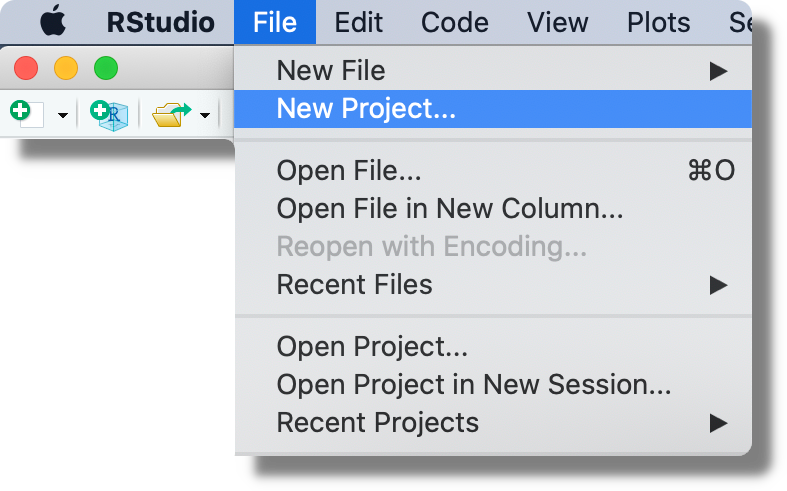
\includegraphics[width=0.6\linewidth]{images/projects/new-proj-1} \end{center}
\item
  When creating a new project, we can decide between starting from a new directory (\emph{``New Directory''}; the most common approach), associating a project with an already existing directory (\emph{``Existing Directory''}), or associating a project to an online repository (\emph{``Version Control''}; for more information see Chapter {[}TODO: add ref{]}).

  \begin{center}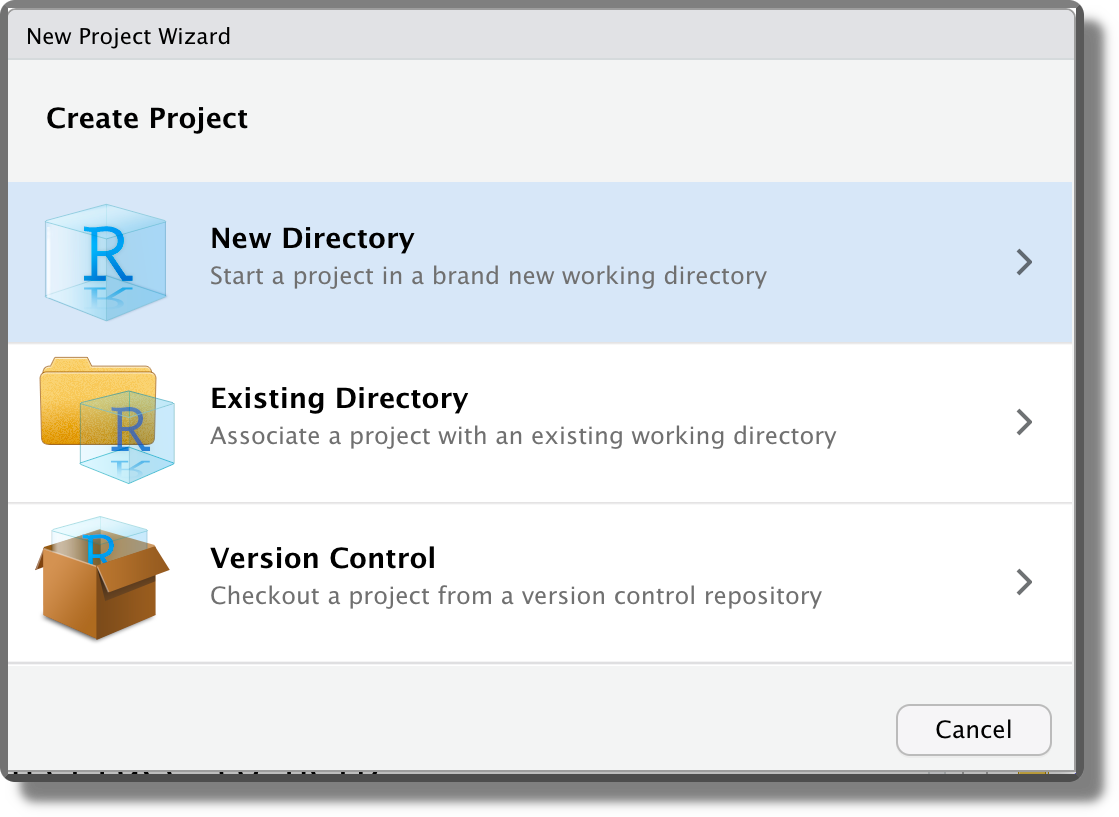
\includegraphics[width=0.6\linewidth]{images/projects/new-proj-2} \end{center}
\item
  Selecting \emph{``New Directory''}, then we can specify the desired project template. Different templates are available also depending on the installed packages. The default option is \emph{``New Project''}.

  \begin{center}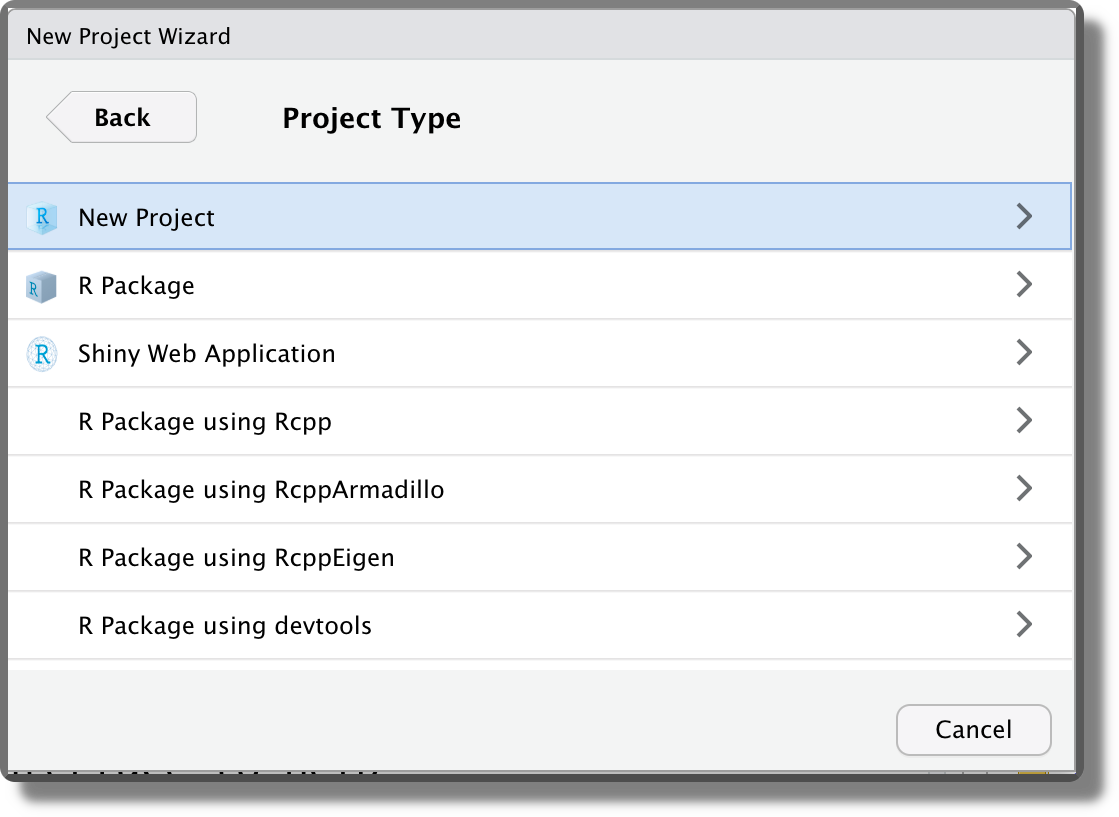
\includegraphics[width=0.6\linewidth]{images/projects/new-proj-3} \end{center}
\item
  Finally, we can indicate the location where to create the project directory and specify the directory name. This will be used also as the project name. Note that two more options are available \emph{``Create a git repository''} and \emph{``Use renv with this project''}. We discuss these options in Chapter {[}TODO: add ref{]}) and Chapter {[}TODO: add ref{]}, respectively.

  \begin{center}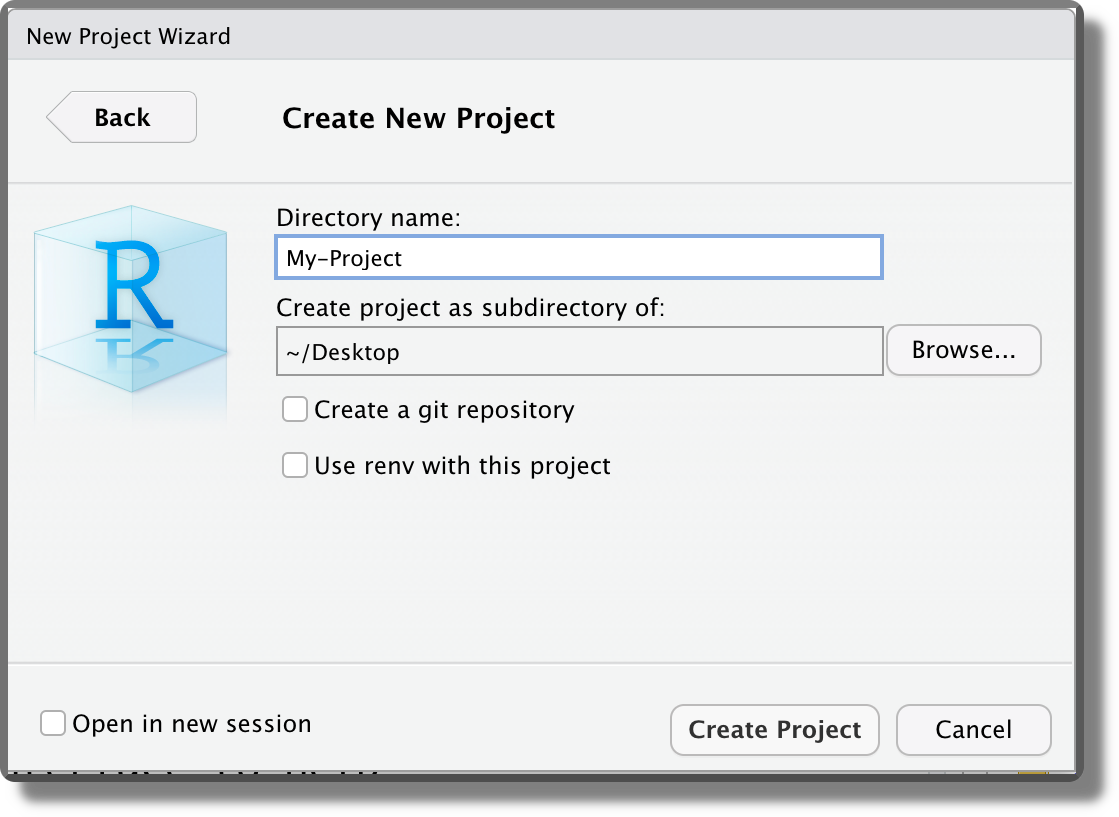
\includegraphics[width=0.6\linewidth]{images/projects/new-proj-4} \end{center}
\item
  Selecting \emph{``Crete Project''}, the project directory is created in the specified location and a new RStudio session is opened. Note that the Rstudio icon now displays the project name currently open 
\includegraphics[width=6.5em,height=\textheight]{images/projects/by-credits.png}. The current project is also indicated in the top right corner. Click on it to see other project options and to close the project (\emph{``Close Project''}; or from the top bar menu \emph{``File -\textgreater{} Close Project''}).

  \begin{center}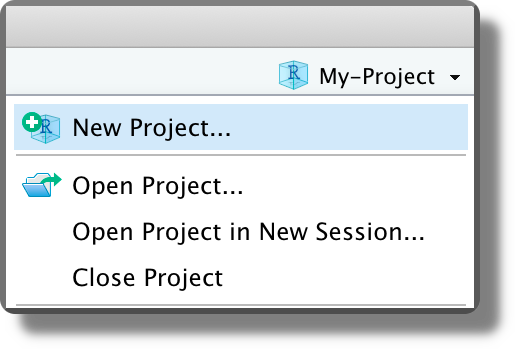
\includegraphics[width=0.4\linewidth]{images/projects/proj-menu} \end{center}
\end{enumerate}

\hypertarget{project-features}{%
\subsection{Project Features}\label{project-features}}

We now discuss the main features of RStudio Projects:

\begin{itemize}
\item
  \textbf{Working Directory and File Paths.} When opening a project, RStudio automatically sets the working directory at the project root. We can check the current working directory by looking at the top of the console panel or using the R command \texttt{getwd()}.

  \begin{center}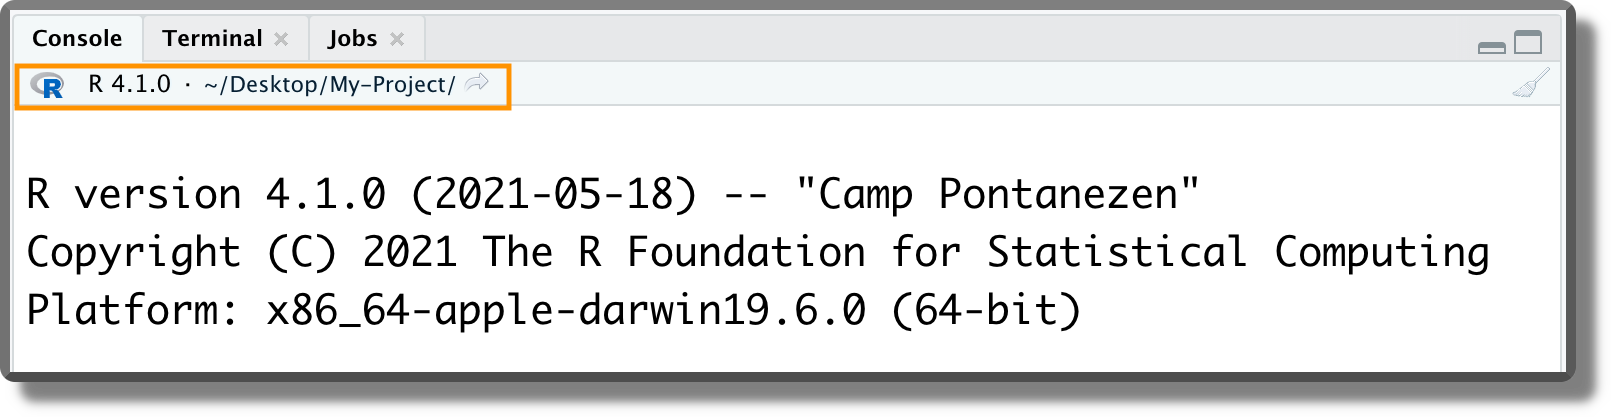
\includegraphics[width=0.9\linewidth]{images/projects/proj-wd} \end{center}

  As discussed in Section \ref{wd-file-path}, this is a very useful feature because now we no longer have to bother about setting the working directory manually (we can finally forget about the \texttt{setwd()} command). Moreover, we can refer to any file using relative paths considering as reference the project root.
\end{itemize}

\begin{design}[File Paths in R]

In R, we can specify file path using forward slash \texttt{"/"} or backslash \texttt{"\textbackslash{}"} independently of the operative system we are currently using. However, the backslash has a special meaning in R as it is used as \emph{escape character}. Thus, to specify a file path using backslash we have to double them (e.g., ``my-project\textbackslash\textbackslash data\textbackslash\textbackslash my-data.csv''). All this leads to a simple solution:

\begin{quote}
Always use forward slash \texttt{"/"} to specify file paths to avoid any troubles (e.g., ``my-project/data/my-data.csv'').
\end{quote}

\end{design}

\begin{itemize}
\item
  \textbf{\texttt{\textless{}project-name\textgreater{}.Rproj} File.} The default Project template creates an empty directory with a single file named \texttt{\textless{}project-name\textgreater{}.Rproj} (plus some hidden files). Clicking on the \texttt{\textless{}project-name\textgreater{}.Rproj} file from the file manager (not from RStudio), we can open the selected project in a new RStudio session. Clicking on the \texttt{\textless{}project-name\textgreater{}.Rproj} file from the file panel in RStudio, instead, we can change the project settings (see the next point). Moreover, from the file panel in RStudio, if we click the Project icon on the top right corner (orange arrow in the image below), we are automatically redirected to the project root.

  \begin{center}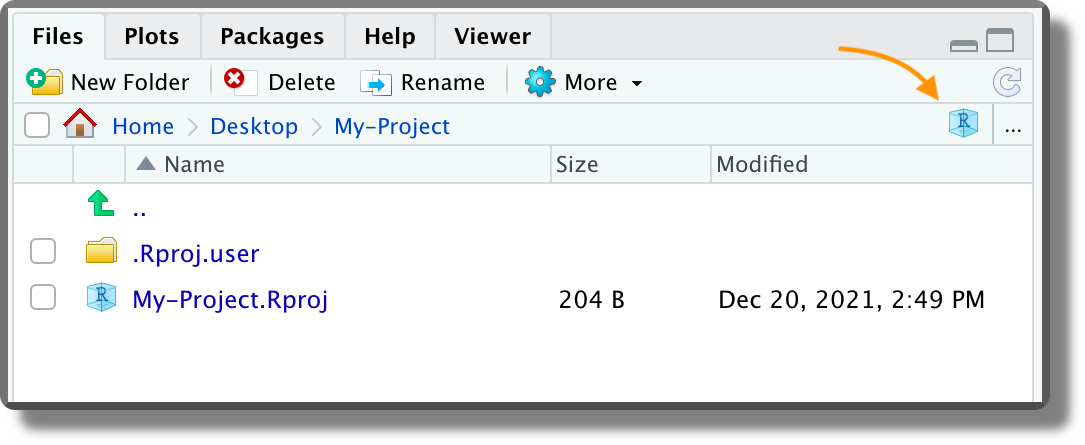
\includegraphics[width=0.6\linewidth]{images/projects/proj-files} \end{center}

  The \texttt{\textless{}project-name\textgreater{}.Rproj} file is simply a text file with the project settings. Using a text editor, we can see the actual content.

  \begin{center}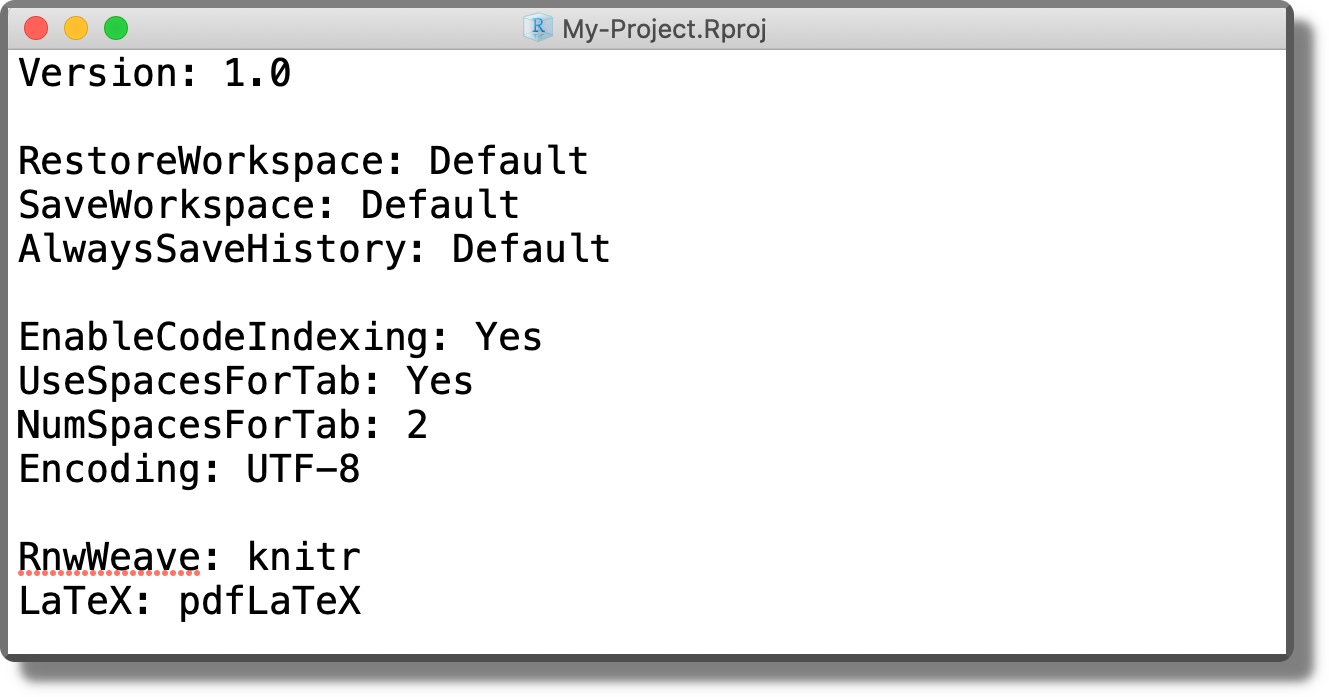
\includegraphics[width=0.6\linewidth]{images/projects/rproj-file} \end{center}
\item
  \textbf{Project Settings.} We can specify specific settings for each project. From the top bar menu, select \emph{``Tools -\textgreater{} Project Options''} and specify the required options according to our needs.

  \begin{center}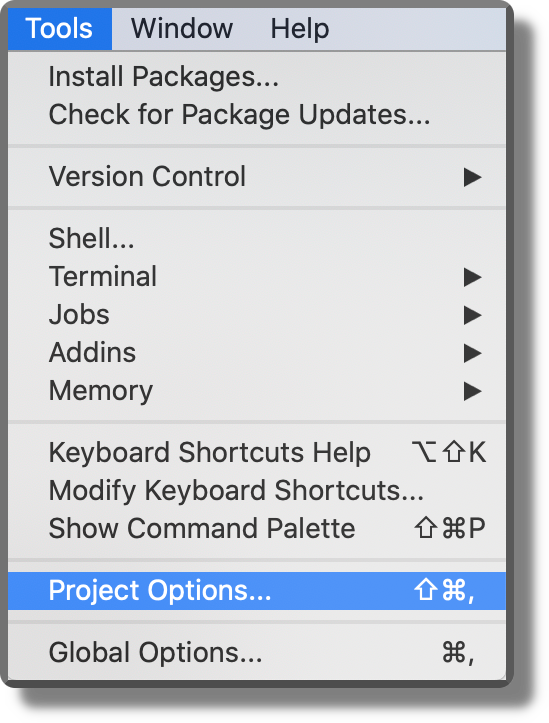
\includegraphics[width=0.4\linewidth]{images/projects/proj-options} \end{center}

  Some recommended settings should be applied as default to all projects. To do that, select from the top bar menu \emph{``Tools -\textgreater{} Global Options''}. From the panel \emph{``General''} in the \emph{``Workspace''} section, ensure the box \emph{``Restore\ldots{}''} is \textbf{not} selected and the option \emph{``Save\ldots{}''} is set to \textbf{Never} (see figure below). This ensures that the workspace is not saved between sessions and every time we start from a new empty environment. The reason for doing this is that it forces us to write everything needed for our project in scripts and then we use scripts to create the required objects. It is a short-term pain for a long-term winning, as it enhances reproducibility and avoids bugs due to overwritten objects in the environment. Moreover, we can finally say goodbye to the horrible \texttt{rm(list=ls())} line of code found at the top of many scripts.

  \begin{center}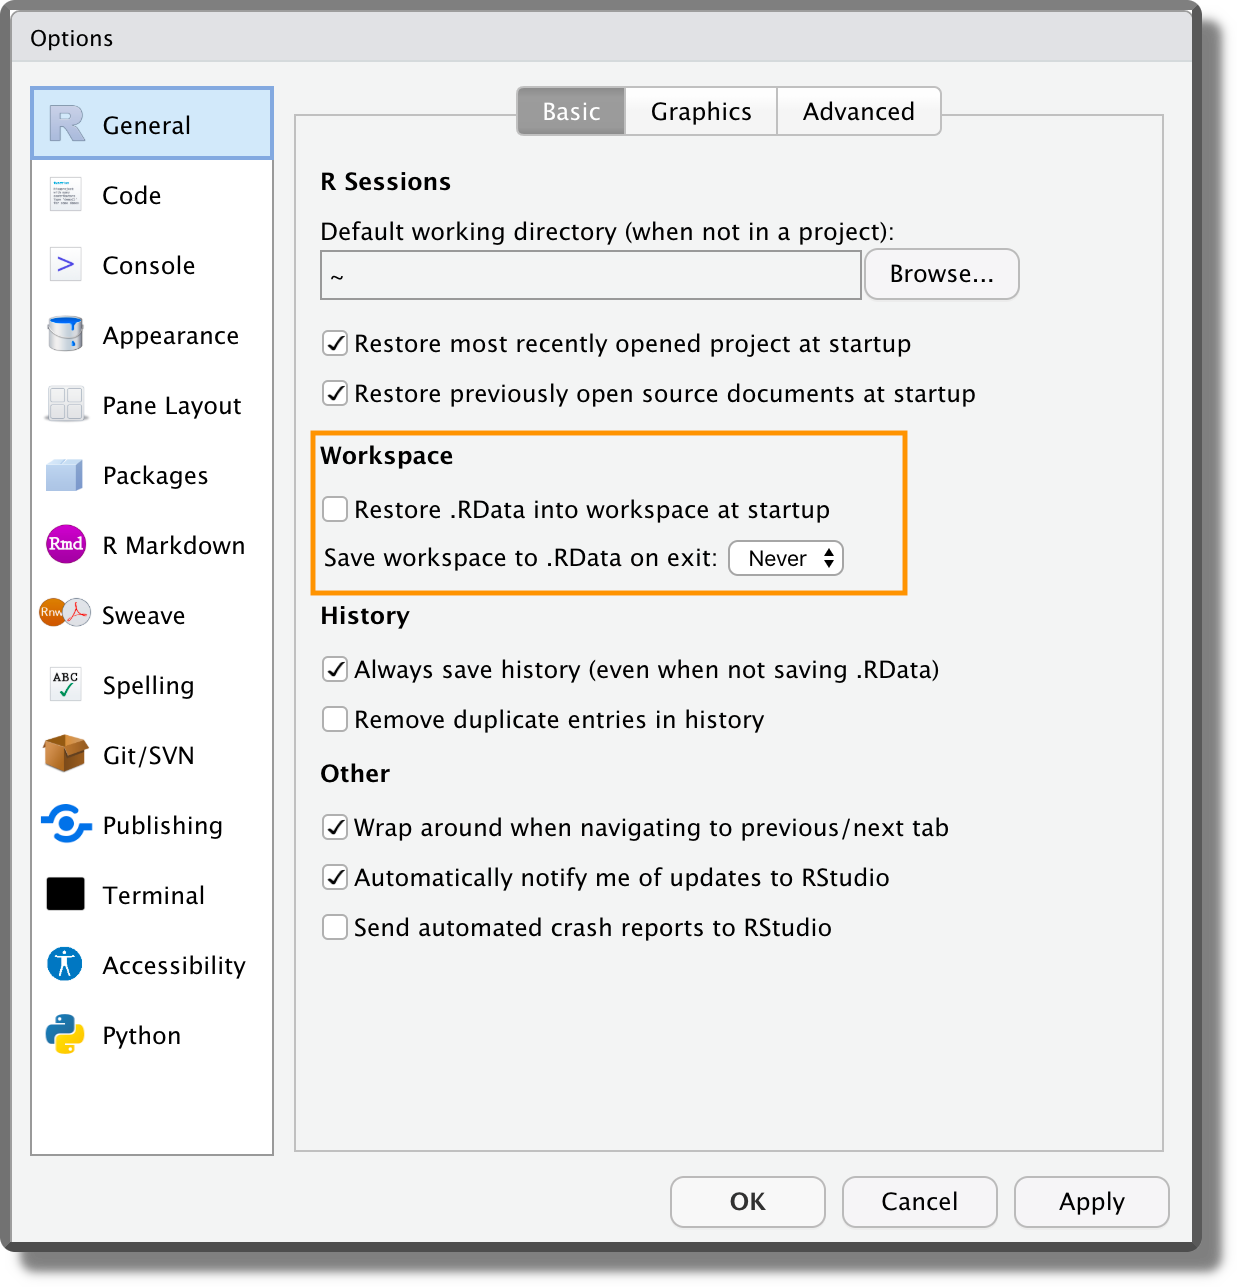
\includegraphics[width=0.6\linewidth]{images/projects/general-options} \end{center}

  Another important setting is the encoding. From the panel \emph{``Code''} ensure that the default text encoding is set to \emph{``UTF-8''}. Encoding defines how the characters are represented by the computer. This could be problematic for different alphabets or special characters (e.g., accented characters). The UTF-8 encoding is becoming the modern standard as it covers all the possibilities.

  \begin{center}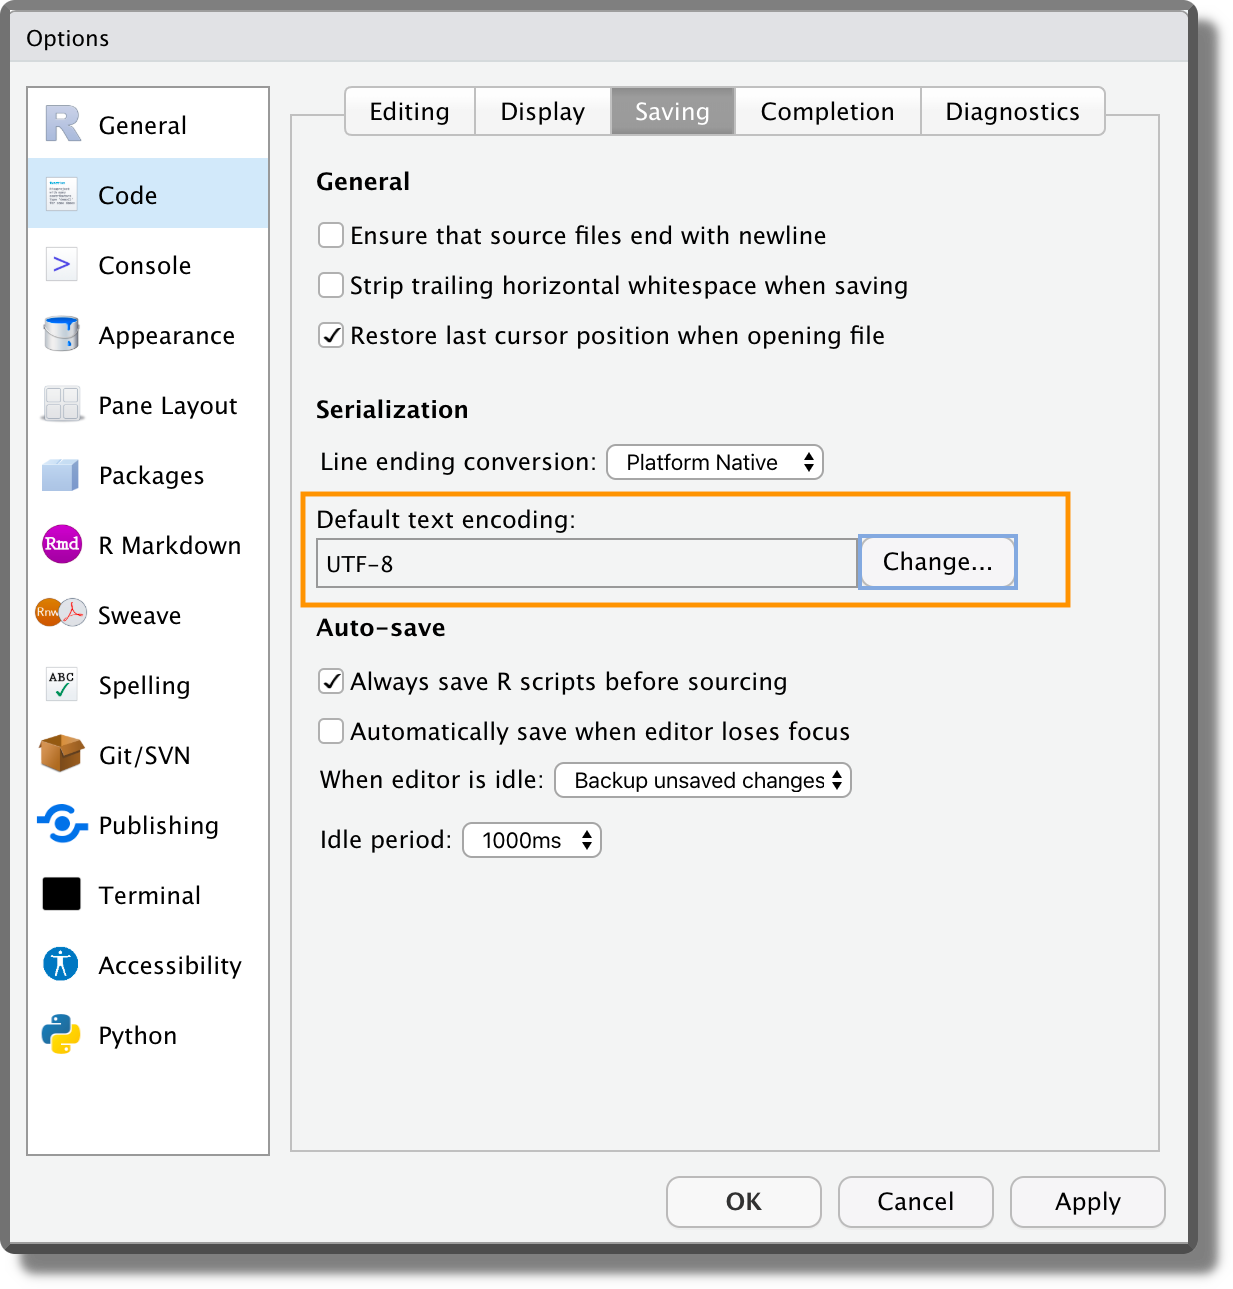
\includegraphics[width=0.6\linewidth]{images/projects/settings-UTF8} \end{center}
\item
  \textbf{\texttt{.Rprofile} File.} This file is a special script that is automatically executed at the beginning of each session (or when the session is restarted). This file is not available by default but we can create it by naming an R script as \texttt{.Rprofile} (\textbf{without extension!}) {[}TODO: check in windows \url{https://stackoverflow.com/questions/28664852/saving-a-file-as-rprofile-in-windows}{]}. Note that names that begin with a dot \texttt{"."} are reserved for the system and are hidden from the file manager. To see the hidden files, select from the files panel in RStudio the option \emph{``Show Hidden Files''}.

  \begin{center}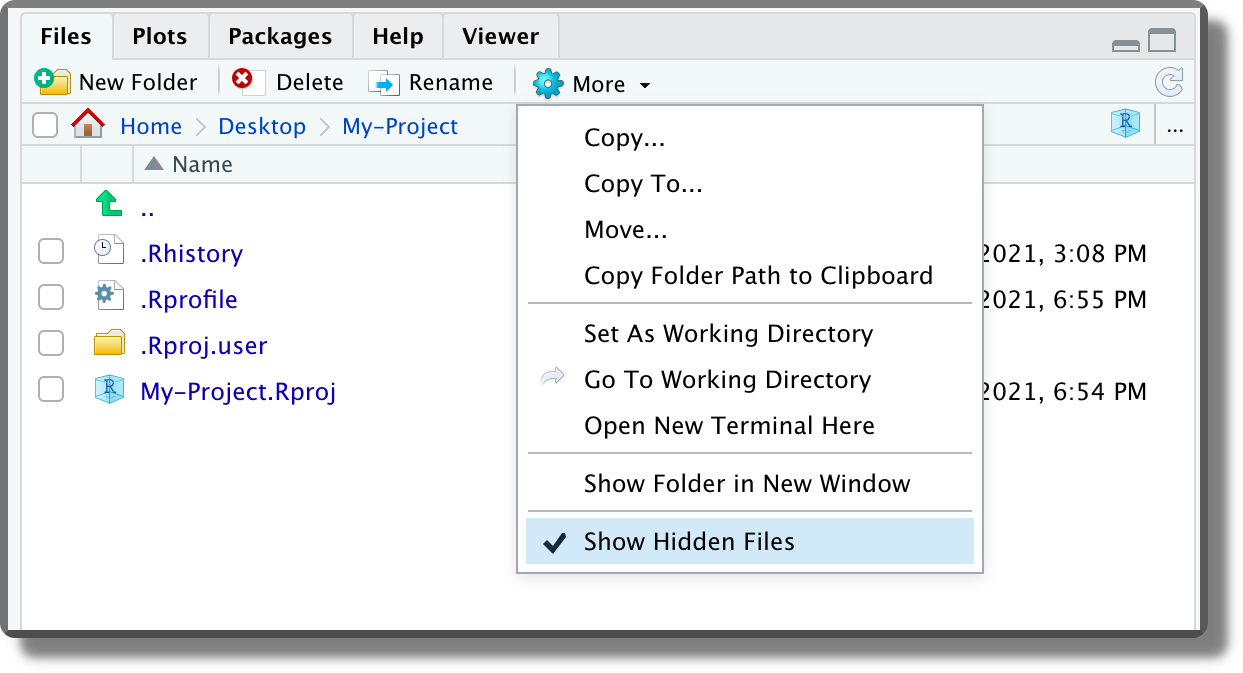
\includegraphics[width=0.6\linewidth]{images/projects/hidden-files} \end{center}

  This file can be used to automate the execution of recurrent operations such as loading the required packages, setting R global options, or other package settings (e.g., ggplot themes). In the example below, we simply set a welcome message.

  \begin{center}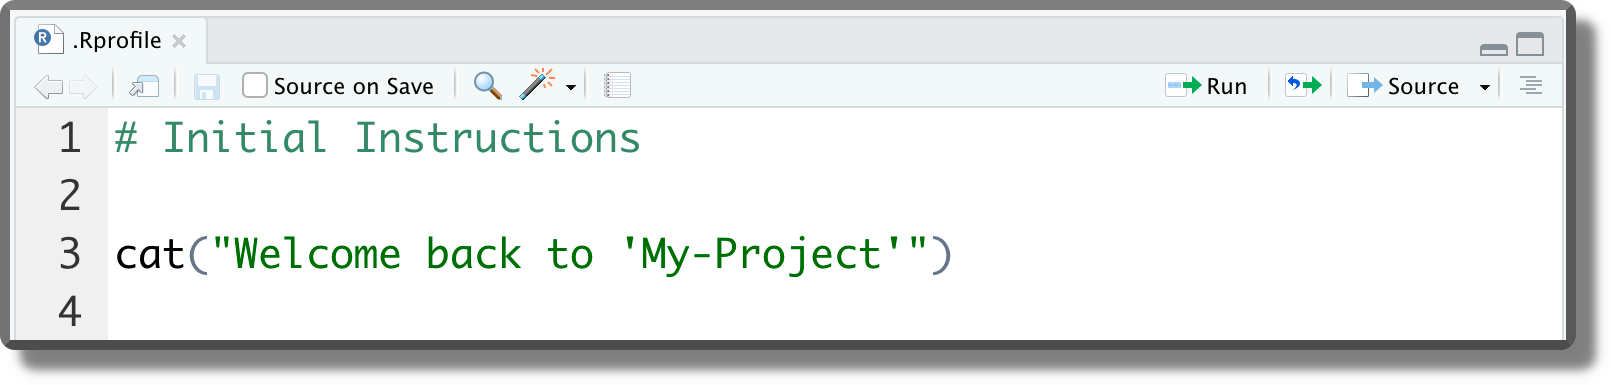
\includegraphics[width=0.6\linewidth]{images/projects/rprofile} \end{center}

  These commands are executed at the beginning of each session or when the session is restarted (\texttt{Ctrl} + \texttt{Shift} + \texttt{F10} on Windows and Linux; \texttt{Cmd/Ctrl} + \texttt{Shift} + \texttt{0} on macOS).

  \begin{center}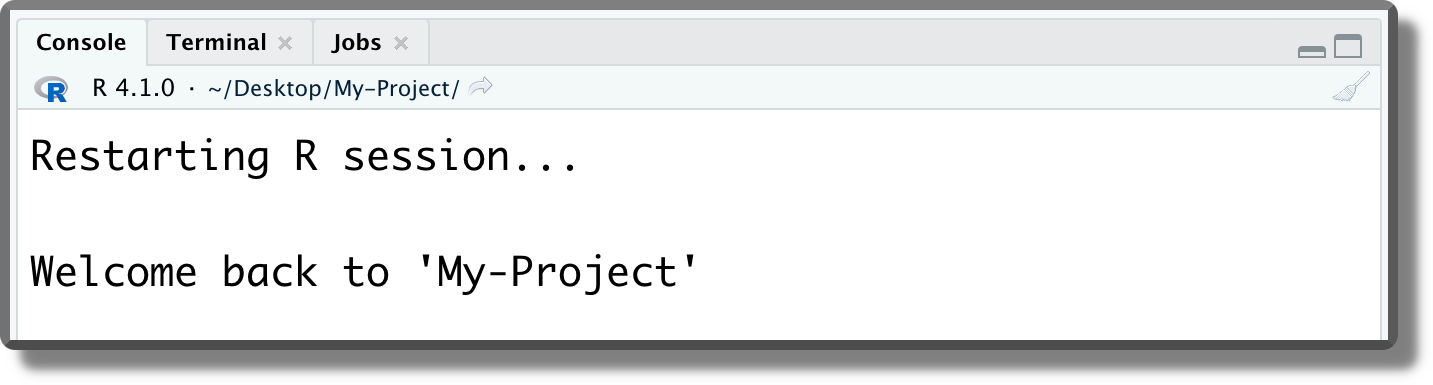
\includegraphics[width=0.6\linewidth]{images/projects/restart-session} \end{center}
\item
  \textbf{Like Multiple Office Desks.} Another advantage of RStudio projects is that we can quickly move from one project to another. When opening a former project, all panels, tabs, and scripts are restored in the same configuration as we left them. This allows us to go straight back into our workflow without wasting any time.

  We can think of it as having a dedicated office desk for each of our projects. On the table, we can leave everything that is required to work on that project and we simply move between different office desks according to the current project we are working on.
\end{itemize}

To know more about RStudio projects, see \url{https://r4ds.had.co.nz/workflow-projects.html}.

\hypertarget{advanced-features}{%
\subsection{Advanced features}\label{advanced-features}}

We briefly point out some other advanced features of RStudio projects. These are covered in more detail in the following Chapters.

\begin{itemize}
\item
  \textbf{R Package Template.} As presented in Section \ref{create-proj}, when creating a new project we can choose different templates. These templates automatically structure the project according to specific needs (e.g., creating a Shiny App or a Bookdown). In particular, one very interesting template is the \emph{R Package Template}.

  The R Package Template is used to create\(\ldots\) guess what? R packages. This template introduces some advanced features of R that become very handy when following a functional style approach. For example, we can manage our project package dependencies, easily load all our functions, document them, and create unit tests. We could go all the way and create a proper R package out of our project that other users can install. This requires some extra work and it may not be worth the effort, but of course, this will depend on the specific project aims.

  Anyway, the R package template is very useful when writing our functions. For this reason, we discuss further details about the R package template in Chapter {[}TODO: add ref{]} when discussing the functional style approach.
\item
  \textbf{Git.} We can use version control systems such as Git to track changes on our RStudio projects. We can decide to create a git repository when creating our new project (see Section \ref{create-proj}) or to associate the project to an existing repository. This is really a huge step forward in the quality of our workflow and it is absolutely worth the initial pain. All the required information to get familiar with Git and how to integrate the git workflow within RStudio projects is presented in Chapter {[}TODO: add ref{]}.
\item
  \textbf{\texttt{renv}.} To allow reproducibility of the result, everyone must use the same project dependencies. This includes not only the specific software and relative packages but also their specific version number. The R packages ecosystem changes quite rapidly, new packages are released every month and already available packages are updated from time to time. This means that in a year or two, our code may fail due to some changes in the underlying dependencies. To avoid these issues, it is important to ensure that the same package versions are always used.

  We could list the required packages in a file and their versions manually or find a way to automate this process. As always, in R there is a package for almost everything and in this case, the answer is \texttt{renv}. \texttt{renv} allows us to manage all the R packages dependencies of our projects in a very smooth workflow. We can include \texttt{renv} in our project when creating a new project (see Section \ref{create-proj}) or add it later. In Chapter {[}TODO: add ref{]}, we introduce all the details about integrating the \texttt{renv} workflow in our projects.
\end{itemize}

\begin{doclinks}

\hypertarget{bibtex}{%
\subsubsection*{Bibtex}\label{bibtex}}
\addcontentsline{toc}{subsubsection}{Bibtex}

\begin{itemize}
\tightlist
\item
  Standard bibtex syntax for bibliography files\newline
  \url{https://www.overleaf.com/learn/latex/Bibliography_management_with_biblatex\#The_bibliography_file}
\end{itemize}

\hypertarget{markown-syntax}{%
\subsubsection*{Markown Syntax}\label{markown-syntax}}
\addcontentsline{toc}{subsubsection}{Markown Syntax}

\begin{itemize}
\tightlist
\item
  Markdown Guide\newline
  \url{https://www.markdownguide.org/}
\end{itemize}

\hypertarget{license-1}{%
\subsubsection*{License}\label{license-1}}
\addcontentsline{toc}{subsubsection}{License}

\begin{itemize}
\tightlist
\item
  Projects with no license\newline
  \url{https://opensource.stackexchange.com/q/1720}
\item
  Differences between GNU and MIT Licenses\newline
  \url{https://www.quora.com/What-are-the-key-differences-between-the-GNU-General-Public-license-and-the-MIT-License}
\item
  Creative Commons license\newline
  \url{https://creativecommons.org/about/cclicenses/}
\item
  Open Science Framework documentation\newline
  \url{https://help.osf.io/hc/en-us/articles/360019739014-Licensing}
\item
  GitHub documentation\newline
  \url{https://docs.github.com/en/repositories/managing-your-repositorys-settings-and-features/customizing-your-repository/licensing-a-repository}
\item
  GitHub license chooser\newline
  \url{https://choosealicense.com/}
\item
  Creative Commons website\newline
  \url{https://creativecommons.org/}
\item
  GitHub Setting a License guide\newline
  \url{https://docs.github.com/en/communities/setting-up-your-project-for-healthy-contributions/adding-a-license-to-a-repository}
\end{itemize}

\hypertarget{paths}{%
\subsubsection*{Paths}\label{paths}}
\addcontentsline{toc}{subsubsection}{Paths}

\begin{itemize}
\tightlist
\item
  Paths in Python\newline
  \url{https://medium.com/@ageitgey/python-3-quick-tip-the-easy-way-to-deal-with-file-paths-on-windows-mac-and-linux-11a072b58d5f}
\end{itemize}

\hypertarget{rstudio-projects-1}{%
\paragraph*{RStudio Projects}\label{rstudio-projects-1}}
\addcontentsline{toc}{paragraph}{RStudio Projects}

\begin{itemize}
\tightlist
\item
  RStudio projects general introduction\newline
  \url{https://r4ds.had.co.nz/workflow-projects.html}
\end{itemize}

\end{doclinks}

\hypertarget{data-chapter}{%
\chapter{Data}\label{data-chapter}}

In the previous chapters, we learned to share our materials through the Open Science Framework (OSF) and to organize all our files in a well structured and documented project.

In this chapter, we focus on data. In particular, in Section \ref{organizing} we provide main guidelines regarding how to organize data inside our project and, in Section \ref{sharing}, we discuss main issues related to sharing data.

\hypertarget{organizing}{%
\section{Organizing Data}\label{organizing}}

Ideally, we want to store all the data relevant to our project in a dedicated directory (e.g., \texttt{data/}). These files should be considered \texttt{read-only} and, in the case of data that required some preprocessing, it is recommended to include also the original raw version of the data or provide a link to retrieve it.

However, storing the data and organising it efficiently is just part of the job. We also need to provide a detailed description with all the information to allow other colleagues (aka the future us) to understand what the data contain. We do not want to save and share useless files full of 0-1 values, right?

Let's discuss how to organize and document our data together with other useful recommendations.

\hypertarget{data-structure}{%
\subsection{Data Structure}\label{data-structure}}

There are many data formats depending on the specific data type (e.g., questionnaires, brain imaging, ERP study, conversations, etc.) and there are often no common standards. Therefore, how to manage and organize data can vary according to the specific case and needs. However, as a general case, we can consider tabular data, that is, data organized in columns and rows.

Tabular data can be structured according to the \emph{wide format} or the \emph{long format}.

\begin{itemize}
\tightlist
\item
  \textbf{Wide Format.} Each variable value is recorded in a separate column.

  \begin{table}[!h]

    \caption{\label{tab:unnamed-chunk-16}Wide Format}
    \centering
    \begin{tabular}[t]{llccc}
    \toprule
    Name & Sex & Age & Pre & Post\\
    \midrule
    Alice & F & 24 & ... & ...\\
    Bob & M & 21 & ... & ...\\
    Carl & M & 23 & ... & ...\\
    \bottomrule
    \end{tabular}
    \end{table}
\item
  \textbf{Long Format.} Multiple variables can be recorded using a column to indicate the name of the measured variable and another column for the measured values.

  \begin{table}[!h]

    \caption{\label{tab:unnamed-chunk-17}Long Format}
    \centering
    \begin{tabular}[t]{llclc}
    \toprule
    Name & Sex & Age & Time & Value\\
    \midrule
    Alice & F & 24 & Pre & ...\\
    Alice & F & 24 & Post & ...\\
    Bob & M & 21 & Pre & ...\\
    Bob & M & 21 & Post & ...\\
    Carl & M & 23 & Pre & ...\\
    \addlinespace
    Carl & M & 23 & Post & ...\\
    \bottomrule
    \end{tabular}
    \end{table}
\end{itemize}

Depending on our specific needs, we may choose a wide or a long format to represent our data. Usually, the long format is the preferred data format, as it is required in most analyses. However, there is an important drawback when using the long format, that is, memory inefficiency.

In general, in a long format dataset, values are unique for each row only for a few columns, whereas for all the other columns the same values are (unnecessarily) repeated multiple times. The Long Format is an inefficient way to store our data.

In the case of small datasets, this does not make a big difference and we can safely continue to store the data using the long format as is the preferred data format in most analyses. When we need to deal with large datasets, however, memory may become a relevant issue. In these cases, we need to find a more efficient way to store our data. For example, we can use the relational model to organize our data.

\begin{itemize}
\item
  \textbf{Relational Model.} Instead of a single large table, the relational model organizes the data more efficiently by using multiple tables. Now, how can we use multiple tables to organize our data more efficiently? To clarify this process, let's consider the data presented in the table above. We have information about participants (i.e., Name, Sex, and Age) and two measures (i.e., Pre and Post) on some outcomes of interest in our study. Using the long data format, participants' information is (unnecessarily) repeated multiple times. Following a relational model, we can create two separate tables, one for the participants' information and the other for the study measures. In this way, we do not repeat the same information multiple times optimizing the memory required to store our data.

  \begin{table}[!h]

    \caption{\label{tab:unnamed-chunk-18}Subjects}
    \centering
    \begin{tabular}[t]{rllr}
    \toprule
    ID & Name & Sex & Age\\
    \midrule
    1 & Alice & F & 24\\
    2 & Bob & M & 21\\
    3 & Carl & M & 23\\
    \bottomrule
    \end{tabular}
    \end{table}

  \begin{table}[!h]

    \caption{\label{tab:unnamed-chunk-18}Study}
    \centering
    \begin{tabular}[t]{cclc}
    \toprule
    ID & Subject\_ID & Time & Value\\
    \midrule
    1 & 1 & Pre & ...\\
    2 & 1 & Post & ...\\
    3 & 2 & Pre & ...\\
    4 & 2 & Post & ...\\
    5 & 3 & Pre & ...\\
    \addlinespace
    6 & 3 & Post & ...\\
    \bottomrule
    \end{tabular}
    \end{table}

  But, how should we read these tables? Note that each table has a column \texttt{ID} with the unique identifier for each row. These IDs are used to define the relational structure between different tables. For example, in our case, the table Study has a column \texttt{Subject\_ID} that indicates the subject ID for that specific row. Matching the \texttt{Subject\_ID} value in the Study table with the \texttt{ID} column in the Subjects table, we can retrieve all the participants' information from a specific row.

  This matching operation is usually defined as a \textbf{JOIN} operation and allows us to reconstruct our data in the desired format starting from separate tables.
\end{itemize}

If you have used SQL before, you are already familiar with relational databases and join operations. At first, these concepts may seem very complicated. In reality, as soon as we familiarize ourselves with all the technical terms, everything becomes very easy and intuitive. So do not be scared by buzz words such as \emph{``primary-key''}, \emph{``foreign-key''}, \emph{``left-join''}, \emph{``inner-join''}, or other jargon. You will quickly master all of them.

Most programming languages provide dedicated libraries and tutorials to execute all these operations. For example, if working with R consider \url{https://r4ds.had.co.nz/relational-data.html}.

\hypertarget{data-docs}{%
\subsection{Documentation}\label{data-docs}}

A dataset without documentation is like a sky without stars\(\ldots\) we can not see anything. We need to describe our data by providing details not only regarding all the variables but also about the data collection process or other information that could be relevant to properly interpret the data.

To document the data, we do not need anything fancy, a simple Markdown file is more than enough. An advantage of using Markdown files is that most online repositories automatically render Markdown files when navigating from the browser.

So, considering the data in the previous example, we could create the following \texttt{data-README.md}.

\begin{Shaded}
\begin{Highlighting}[]
\CommentTok{\#{-}{-}{-}{-}{-}     data{-}README.md    {-}{-}{-}{-}\#}

\CommentTok{\# Data README}

\CommentTok{\#\# General Info }

\ExtensionTok{Details}\NormalTok{ about the study/project, authors, License, or other relevant }
\ExtensionTok{information.}

\ExtensionTok{Description}\NormalTok{ of the data collection process or links to the paper/external }
\ExtensionTok{documentation}\NormalTok{ for further details.}

\CommentTok{\#\# Details}

\ExtensionTok{The}\NormalTok{ dataset }\KeywordTok{\textasciigrave{}}\ExtensionTok{my{-}study.csv}\KeywordTok{\textasciigrave{}}\NormalTok{ is formed by n rows and k columns:}

\ExtensionTok{{-}} \KeywordTok{\textasciigrave{}}\ExtensionTok{Name}\KeywordTok{\textasciigrave{}}\NormalTok{. Character variable indicating the subject name}
\ExtensionTok{{-}} \KeywordTok{\textasciigrave{}}\ExtensionTok{Sex}\KeywordTok{\textasciigrave{}}\NormalTok{. Factor variable indicating the subject gender }\ErrorTok{(}\ExtensionTok{levels}\NormalTok{ are }\KeywordTok{\textasciigrave{}}\StringTok{"F"}\KeywordTok{\textasciigrave{}} 
         \ControlFlowTok{for}\NormalTok{ females }\ExtensionTok{and} \KeywordTok{\textasciigrave{}}\StringTok{"M"}\KeywordTok{\textasciigrave{}}\NormalTok{ for males}\KeywordTok{)}
\ExtensionTok{{-}} \KeywordTok{\textasciigrave{}}\ExtensionTok{Age}\KeywordTok{\textasciigrave{}}\NormalTok{. Numeric variable indicating subject age }\ErrorTok{(in} \ExtensionTok{years}\KeywordTok{)}
\ExtensionTok{{-}} \KeywordTok{\textasciigrave{}}\ExtensionTok{Time}\KeywordTok{\textasciigrave{}}\NormalTok{. Factor variable indicating measure time }\ErrorTok{(}\ExtensionTok{levels}\NormalTok{ are }\KeywordTok{\textasciigrave{}}\StringTok{"Pre"}\KeywordTok{\textasciigrave{}}\NormalTok{ and}
          \KeywordTok{\textasciigrave{}}\StringTok{"Post"}\KeywordTok{\textasciigrave{})}
\ExtensionTok{{-}} \KeywordTok{\textasciigrave{}}\ExtensionTok{Value}\KeywordTok{\textasciigrave{}}\NormalTok{. Numeric variable indicating the outcome measure}
\ExtensionTok{{-}}\NormalTok{ ...}
\end{Highlighting}
\end{Shaded}

There are no strict rules about what we should include or not in our data README file. We are free to structure it according to our needs. As a generic recommendation, however, we should specify data general information about:

\begin{itemize}
\tightlist
\item
  \textbf{Study/Project.} Reference to the specific study or project.
\item
  \textbf{Authors.} List of the authors with contact details of the corresponding author or the maintainer of the project.
\item
  \textbf{License.} Specify under which license the data are released (see Section \ref{license-data}).
\item
  \textbf{Data Collection Process.} Description of relevant aspects of the data collection or external links for further details.
\end{itemize}

Ideally, we should provide all the required details to allow other colleagues to understand the context in which data were collected and to evaluate their relevance for possible other uses (e.g., meta-analyses). We can also provide links to raw data if these are available elsewhere.

Considering the information about the dataset, we should provide the dimension of the dataset and a list with the details for each variable. In particular, we should indicate:

\begin{itemize}
\tightlist
\item
  \textbf{Variable Name.} The name of the variable as it is coded.
\item
  \textbf{Variable Type.} The specific variable type (i.e., string, integer, numeric, logic, other)
\item
  \textbf{Variable Meaning.} The description of what the values indicate.
\item
  \textbf{Variable Values.} Information about the variable values. This could include a list of all the labels and their meaning (or the number of levels) for categorical variables; the range of allowed values for numeric variables; the unit of measurement or a description of how the variable was computed if relevant.
\item
  \textbf{Missing Values.} Specify how missing values are coded or any other value used to indicate special conditions.
\end{itemize}

\hypertarget{data-good-practices}{%
\subsection{Data Good Practices}\label{data-good-practices}}

Finally, let's consider two other general aspects regarding data that are important to take into account:

\begin{itemize}
\item
  \textbf{File Format.} There are many possible file formats. However, an important distinction concerns proprietary format and open format (definitions adapted from the Open Data Handbook, see \url{https://opendatahandbook.org}).

  \textbf{Proprietary Format.} Those formats owned and controlled by a specific company. These data formats require specific dedicated software to be read reliably and usually, we need to pay to use them. Note that the description of these formats may be confidential or unpublished, and can be changed by the company at any time. Common examples are XLS and XLSX formats used by Microsoft Excel.

  \textbf{Open Format.} All those file formats that can be reliably used by at least one free/open-source software tool. A file in an open format guarantees that there are no restrictions or monetary fee to correctly read and use it. Common examples are the \texttt{RDA} and \texttt{RDS} formats used internally by R.

  We should avoid proprietary formats and always use open formats, instead. In particular, we should not use open formats related to specific software (even if is open-source), but prefer general text formats (e.g., CSV) that can be used easily by many tools.
\item
  \textbf{Machine Readable.} Data should be stored in a format that allows other researchers to easily use them. People saving tabular data in a PDF file would deserve to be punished in hell. Do they expect us to copy and paste all values by hand?
\item
  \textbf{Character Encoding.} All characters (i.e., letters, numbers and symbols) are stored in our machine as sequence bits (i.e., the fundamental unit of information that can assume binary values 0 or 1). Encoding refers to the specific process of converting different characters into their numerical representation. While decoding is the reverse operation.

  There are different standards for different alphabets, so if we open a text file using the wrong decoding, characters can be confused with each other. Many issues typically arise with accented letters.

  \textbf{UTF-8} is becoming the standard method for encoding files, as it allows to encode efficiently all characters from any alphabet. We should always save our data and any other file using the UTF-8 encoding. If for some reason we need to use a different encoding, remember to explicitly state the used encoding. This will save our colleagues from lots of trouble.

  From RStudio, we can set UTF-8 as default text encoding from \emph{``Tools -\textgreater{} Global Options -\textgreater{} Code -\textgreater{} Saving''}.

  \begin{center}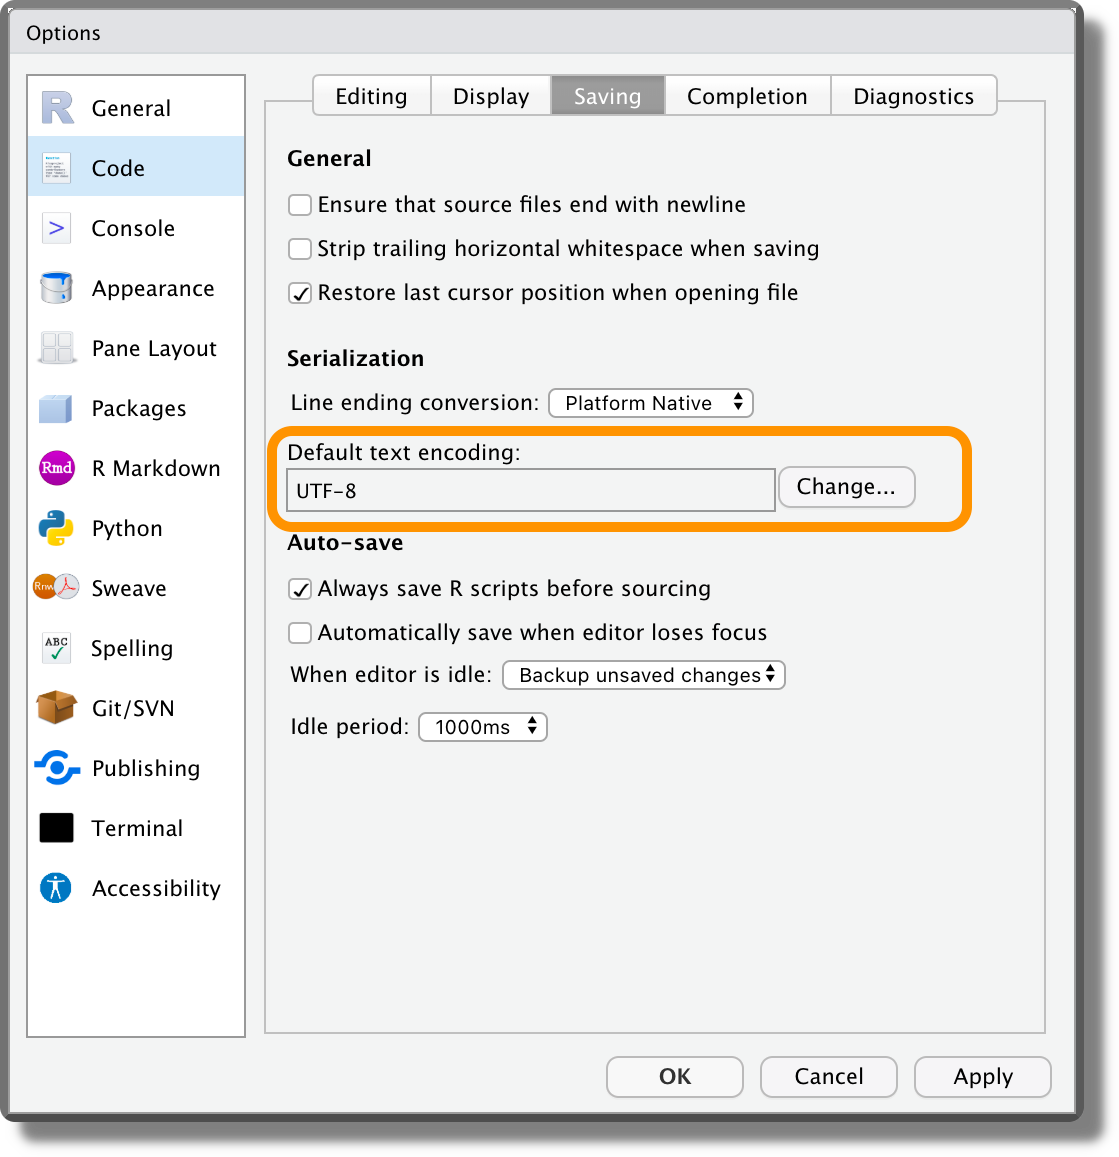
\includegraphics[width=0.7\linewidth]{images/data/encoding} \end{center}
\item
  \textbf{The Rawer the Better.} We should share data in a format as raw as possible allowing other colleagues to reproduce the analysis from the very beginning.
\end{itemize}

\hypertarget{sharing}{%
\section{Sharing Data}\label{sharing}}

The most important part of our studies is not our conclusions but our data. Of course, this is a very provocative claim, but there is some truth in it. Making data available allows other researchers to build upon previous work leading to the efficient incremental development of the scientific field. For these reasons, we should always share our data.

Imagine we came up with a new idea. If we have access to many datasets relevant to the topic, we could immediately test our hypotheses. This would allow us to refine our hypotheses and properly design a new experiment to clarify possible issues. Wouldn't this be an ideal process?

Of course, one of the main resistance to sharing data is that data collection is extremely costly in terms of time, effort and money. Therefore, we may feel reluctant to share something that cost us so much and from which others can take all the merits if they come up with a new finding. Unfortunately, in today's hyper-competitive \emph{``publish or perish''} world, the spotlight only shines on who comes with the new ideas neglecting the fundamental contribution of those who collected the data that made all this possible. Hopefully, in the future, the merit of both will be recognized.

Regarding this topic, there is a famous historical anecdote. Almost anyone knows or at least has heard Kepler's name. Johannes Kepler (1571 -- 1630) was a German astronomer and mathematician who discovered that the orbits of planets around the Sun are elliptical and not circular as previously thought. This was an exceptional claim that earned him eternal fame with Kepler's laws of planetary motion (\url{https://en.wikipedia.org/wiki/Kepler\%27s_laws_of_planetary_motion}). However, fewer people know the name of Brahe. Tycho Brahe (1546 - 1601) was a Danish astronomer, known for his accurate and comprehensive astronomical observations. Kepler became Brahe's assistant and thanks to Brahe's observational data was able to develop his theory about planetary motion. Of course, any researcher would like to become the next Kepler with an eternal law in our name, but who knows, we might as well as be remembered for our data. Do not waste the opportunity of being the next Brahe!

So, after this historical excursus, let's go back to the present and discuss relevant aspects of sharing data.

\hypertarget{when-where-who}{%
\subsection{When, Where, Who?}\label{when-where-who}}

Let's consider some common questions about sharing data:

\begin{itemize}
\item
  \textbf{When to Share?.} From a user point of view, probably the best timing is when the reference article goes to press. In this way, we try to get the best out of our valuable data but we also make them available so other researchers can build upon our work.

  We can also share data and materials in a private mode, granting access to selected people (e.g., reviewers) before the publication, and unlocking the public access in a second moment.

  However, some restrictions can arise from the legal clauses of the research grants or other legal aspects. If we are not allowed to share the data, we should at least justify the reasons (e.g., privacy issues, national security secrets).
\item
  \textbf{Where to Share?.} We need to store materials in an online repository and provide the link to the repository and related research papers that are based on these materials.

  Ideally, we will collect everything in a single place. However, we could also store them in multiple places, to get the advantage of services with appropriate features for specialized types of data or materials. In this case, we should choose a central hub and provide links to other repositories. Of course, this increases the effort required to organize and maintain the project.

  There are many services that allow us to share our material and provide many useful features. For example:

  \begin{itemize}
  \tightlist
  \item
    
\includegraphics[width=9.5em,height=\textheight]{images/projects/by-credits.png} (\url{https://osf.io})
  \item
    
\includegraphics[width=10.5em,height=\textheight]{images/projects/by-credits.png} (\url{https://github.com})
  \item
    
\includegraphics[width=11.5em,height=\textheight]{images/projects/by-credits.png} (\url{https://gitlab.com})
  \item
    
\includegraphics[width=12.5em,height=\textheight]{images/projects/by-credits.png} (\url{https://dataverse.org})
  \item
    
\includegraphics[width=8.5em,height=\textheight]{images/projects/by-credits.png} (\url{https://nyu.databrary.org})
  \item
    
\includegraphics[width=9.5em,height=\textheight]{images/projects/by-credits.png} (\url{https://www.icpsr.umich.edu})
  \end{itemize}

  Moreover, there could be dedicated services for specific scientific fields or data types.
\item
  \textbf{With whom to share?} Data need not be necessarily made available to everybody to meet open-science standards.

  Many online services allow us to select with whom to share our data. For example, Databrary allows different Release Levels for sharing data: Private (data are available only to the research team); authorized users (data are available to authorized researchers and their affiliates); public (data are available openly to anyone).
\end{itemize}

\hypertarget{legal-aspects}{%
\subsection{Legal Aspects}\label{legal-aspects}}

Specific legal restrictions related to data sharing change from state to state. Therefore, here we only discuss the general recommendation and we should always ensure to abide by our local legal restrictions.

\begin{itemize}
\item
  \textbf{Informed Consent and Permission to Share.} Participants should be informed about the study (e.g.~purposes, approval by an ethics committee), what the risks are, and their rights (e.g.~to leave the study). We need both, participants' consent to participate in the research study and participants' permission to share their research data.

  Note that these are two different things and the best practice for permission to share data is to seek it after the completion of research activities. This ensures that participants are fully aware of the study's procedures and what they are being asked to share.
\item
  \textbf{Data Subject to Privacy Rules.} When sharing data we need to pay special attention to:

  \begin{itemize}
  \tightlist
  \item
    \textbf{Personal data} is information making a person identifiable.
  \item
    \textbf{Sensitive data} are personal data revealing racial or ethnic origin, religious and philosophical beliefs, political opinions, labour union membership, health, sex life and sexual orientation, and genetic and biometric data.
  \item
    \textbf{Legal data} are another type of personal data on which put attention
  \item
    \textbf{Other data} such as private conversations, geolocalization, etc., also require special attention.
  \end{itemize}
\item
  \textbf{Data Anonymization.} Pseudonymisation or removing any information that could be used to identify participants is necessary before sharing the data.
\item
  \textbf{Geographical Restrictions.} {[}TODO: check{]} The GDPR requires that all data collected on citizens must be either stored in the EU, so it is subject to European privacy laws, or within a jurisdiction that has similar levels of protection.
\end{itemize}

\hypertarget{license-data}{%
\subsection{License}\label{license-data}}

As discussed in Chapter \ref{license-section}, specifying a license is important to clarify under which conditions other colleagues can copy, share, and use our project. Without a license, our project is under exclusive copyright by default. Therefore, we always need to add a license to our project.

The same applies to data. In addition to the \emph{Creative Commons Licenses} presented in Chapter \ref{license-section}, there are also other licenses specific for data/databases published by the \textbf{Open Data Commons}, part of the Open Knowledge Foundation.

A database right is a sui generis property right, that exists to recognise the investment that is made in compiling a database, even when this does not involve the ``creative'' aspect that is reflected by copyright (from Wikipedia; \url{https://en.wikipedia.org/wiki/Database_right}).

The main Open Data Commons Licenses are

\begin{itemize}
\tightlist
\item
  \textbf{ODC-BY.} Open Data Commons Attribution License requiring Attribution.
\item
  \textbf{ODbL.} Open Data Commons Open Database License requiring Attribution and Share-alike.
\item
  \textbf{PDDL.} Open Data Commons Public Domain Dedication and License dedicated to the Public Domain (all rights waived).
\item
  \textbf{DbCL.} Database Content License requiring Attribution/Share-alike.
\end{itemize}

Note that Open Data Commons licenses distinguish between \emph{``database''} and \emph{``content''}.
Why distinguish? Image a database of images\(\ldots\)When licensing data, you need to know if the content of the database is homogeneous in terms of the license, or not, and to license accordingly.

{[}TODO: ?? expand{]}

For all the details about licenses dedicated to open data and how to apply them, see \url{https://opendefinition.org/licenses/}.

\hypertarget{metadata}{%
\subsection{Metadata}\label{metadata}}

Finally, to really be open, data must be findable as well. All our effort will be wasted if no one can find our data. However, just sharing the links of an online repository could not be enough. We need to make our data findable by research engines for datasets such as Google Dataset Search (\url{https://datasetsearch.research.google.com}).

To do that, our data needs to be formatted according to a machine-readable format. Moreover, we need to provide the required metadata. Metadata is information about the data going with main data tables. In particular, we have:

\begin{itemize}
\tightlist
\item
  \textbf{Data Dictionary:} a document detailing the information provided by data (e.g.~the type of data, the author);
\item
  \textbf{Codebook:} if necessary, a document describing decoding rules for encoded data (e.g.~0=female / 1=male, Likert descriptors).
\end{itemize}

These documents are similar to what we described in Section \ref{data-docs}. However, before we created human-readable reports, now we need to structure these files in a machine-readable format.

Two data formats that are machine-readable (but also fairly human-readable) are the \emph{eXtensible Markup Language} (XML) and the \emph{JavaScript Object Notation} (JSON) formats.

These topics are beyond the aim of the present chapter. However, the \emph{``Getting Started Creating Data Dictionaries: How to Create a Shareable Data Set''} tutorial by \protect\hyperlink{ref-buchananGettingStartedCreating2021}{Buchanan et al.} (\protect\hyperlink{ref-buchananGettingStartedCreating2021}{2021}) provides a detailed guide to creating dictionaries and codebooks for sharing machine-readable data.

In particular, they cover the use of:

\begin{itemize}
\tightlist
\item
  \textbf{JSON-Linked Data} (JSON-LD), a format designed specifically for metadata.
\item
  \textbf{Schema.org} (\url{https://schema.org/}), a collaborative, community activity with a mission to create, maintain, and promote schemas for structured data on the Internet.
\end{itemize}

The combination of JSON-LD and Schema.org allows the creation of machine-readable data optimized for search engines.

\begin{doclinks}

\hypertarget{relational-data}{%
\subsubsection*{Relational Data}\label{relational-data}}
\addcontentsline{toc}{subsubsection}{Relational Data}

\begin{itemize}
\tightlist
\item
  Relational Data in R\newline
  \url{https://r4ds.had.co.nz/relational-data.htm}
\end{itemize}

\hypertarget{open-data}{%
\subsubsection*{Open Data}\label{open-data}}
\addcontentsline{toc}{subsubsection}{Open Data}

\begin{itemize}
\tightlist
\item
  Open Data Handbook\newline
  \url{https://opendatahandbook.org/}
\item
  Google Dataset Search\newline
  \url{https://datasetsearch.research.google.com/}
\end{itemize}

\hypertarget{repository-platforms}{%
\subsubsection*{Repository Platforms}\label{repository-platforms}}
\addcontentsline{toc}{subsubsection}{Repository Platforms}

\begin{itemize}
\tightlist
\item
  The Open Science Framework (OSF)\newline
  \url{https://osf.io}
\item
  GitHub\newline
  \url{https://github.com}
\item
  GitLab\newline
  \url{https://gitlab.com}
\item
  The Dataverse Project\newline
  \url{https://dataverse.org}
\item
  Databrary\newline
  \url{https://nyu.databrary.org}
\item
  Inter-university Consortium for Political and Social Research (ICPSR)\newline
  \url{https://www.icpsr.umich.edu}
\end{itemize}

\hypertarget{license-open-data}{%
\subsubsection*{License Open Data}\label{license-open-data}}
\addcontentsline{toc}{subsubsection}{License Open Data}

\begin{itemize}
\tightlist
\item
  Database Rights\newline
  \url{https://en.wikipedia.org/wiki/Database_right}
\item
  Conformant License\newline
  \url{https://opendefinition.org/licenses/}
\end{itemize}

\hypertarget{metadata-1}{%
\subsubsection*{Metadata}\label{metadata-1}}
\addcontentsline{toc}{subsubsection}{Metadata}

\begin{itemize}
\tightlist
\item
  \emph{``Getting Started Creating Data Dictionaries: How to Create a Shareable Data Set''} \protect\hyperlink{ref-buchananGettingStartedCreating2021}{Buchanan et al.} (\protect\hyperlink{ref-buchananGettingStartedCreating2021}{2021}) \newline
  \url{https://doi.org/10.1177/2515245920928007}
\item
  Schema.org\newline
  \url{https://schema.org/}
\end{itemize}

\end{doclinks}

\hypertarget{references}{%
\chapter*{References}\label{references}}
\addcontentsline{toc}{chapter}{References}

\hypertarget{refs}{}
\begin{CSLReferences}{1}{0}
\leavevmode\vadjust pre{\hypertarget{ref-buchananGettingStartedCreating2021}{}}%
Buchanan, E. M., Crain, S. E., Cunningham, A. L., Johnson, H. R., Stash, H., Papadatou-Pastou, M., Isager, P. M., Carlsson, R., \& Aczel, B. (2021). Getting {Started Creating Data Dictionaries}: {How} to {Create} a {Shareable Data Set}. \emph{Advances in Methods and Practices in Psychological Science}, \emph{4}(1), 2515245920928007. \url{https://doi.org/10.1177/2515245920928007}

\leavevmode\vadjust pre{\hypertarget{ref-nosekWhatReplication2020}{}}%
Nosek, B. A., \& Errington, T. M. (2020). What is replication? \emph{PLOS Biology}, \emph{18}(3), e3000691. \url{https://doi.org/10.1371/journal.pbio.3000691}

\end{CSLReferences}

\end{document}
